
\documentclass[oneside,12pt]{book}

\usepackage[utf8]{inputenc}
\usepackage[greek, english]{babel}

% Packages
\usepackage{alphabeta}
\usepackage{amsmath}
\usepackage{amsthm}
\usepackage{caption}
\usepackage{color}
\usepackage{fullpage}
\usepackage{graphicx}
\usepackage{latexsym}
\usepackage{listings}
\usepackage{pxfonts}
\usepackage{stackrel}
\usepackage{titlesec}
\usepackage{subfig}
\usepackage{tikz}
\usepackage{float}
\usepackage{hyperref}
\usepackage{setspace}
\usepackage{tcolorbox}
\usepackage[ruled,vlined]{algorithm2e}
\tcbuselibrary{theorems}

\addto{\captionsenglish}{\renewcommand{\bibname}{}}
\patchcmd{\thebibliography}{\chapter*}{\section*}{}{}

\newtcbtheorem[number within=section]{mydefinition}{Ορισμός}%
{colback=black!5,colframe=black!15!black,fonttitle=\bfseries}{th}

\newtcbtheorem[number within=section]{mytheorem}{Θεώρημα}%
{colback=black!5,colframe=black!15!black,fonttitle=\bfseries}{th}

\newtcbtheorem[number within=section]{mylemma}{Λήμμα}%
{colback=black!5,colframe=black!15!black,fonttitle=\bfseries}{th}

% Commands
\newcommand{\N}{\mathbb{N}}
\newcommand{\R}{\mathbb{R}}
\newcommand{\code}[2]{\lstinputlisting[caption={#2}]{#1}}
\newcommand{\margin}{\hspace{4pt}}
\newcommand{\norm}[1]{\left\lVert#1\right\rVert}
\newcommand{\abs}[1]{\left\lvert#1\right\rvert}

% Environments
\newenvironment{matlab}
	{\begin{figure}[hp]\centering\captionsetup{justification=centering}}
	{\end{figure}}

\newenvironment{rcases}
	{\left.\begin{aligned}}
	{\end{aligned}\right\rbrace}
% Python Syntax Highlighting
\definecolor{string_color}{RGB}{0, 161, 13}
\definecolor{comment_color}{RGB}{46, 46, 46}
\definecolor{keyword_color}{RGB}{0, 112, 191}
\definecolor{background_color}{RGB}{250, 250, 250}
\lstset{
    framesep=15pt,
    xleftmargin=15pt,
    xrightmargin=15pt,
    language=Python,
    captionpos=b,
    numbers=right,
    numberstyle=\small\ttfamily,
    frame=lines,
    showspaces=false,
    showtabs=false,
    breaklines=true,
    showstringspaces=false,
    breakatwhitespace=true,
    commentstyle=\color{comment_color}\textit,
    keywordstyle=\bfseries\color{keyword_color}\textbf,
    stringstyle=\color{string_color}\textit,
    morekeywords={self, lambda, __init__, __del__, __name__, for, in, not, and, or, :},
    basicstyle=\small\ttfamily,
    tabsize=4,
    keepspaces=true,
    columns=flexible,
    backgroundcolor=\color{background_color}
}
% Links
\hypersetup{
    colorlinks=true,
    linkcolor=blue,
    filecolor=magenta,
    urlcolor=cyan,
}
% Lengths
\setlength{\parindent}{0in}
\setlength{\oddsidemargin}{0in}
\setlength{\textwidth}{6.5in}
\setlength{\textheight}{10in}
\setlength{\topmargin}{-1.0in}
\setlength{\headheight}{18pt}
\setlength{\parskip}{0.3cm}
\setlength{\parindent}{5ex}
\doublespacing
\theoremstyle{definition}
\newtheorem{definition}{Definition}[section]
\titlespacing*{\subsection}
{0pt}{5.5ex plus 1ex minus .2ex}{4.3ex plus .2ex}
\title{\huge Travelling Salesman Problem}
\author{Σιώρος Βασίλειος\\Ανδρινοπούλου Χριστίνα}
\date{Μάϊος 2020}
\begin{document}
\maketitle
\pagenumbering{gobble}
\pagebreak
\tableofcontents

\chapter{Abstract}

\chapter{Introduction}

Το "Travelling Salesman Problem" (TSP) ή με την ελληνική του απόδοση "Πρόβλημα του πλανόδιου πωλητή" (ή εναλλακτικά πρόβλημα του περιοδεύοντος πωλητή) είναι ένα κλασσικό πρόβλημα θεωρητικής επιστήμης των  υπολογιστών. Πρόκειται για ένα πρόβλημα περιήγησης. Ο πωλητής οφείλει να επισκευτεί n το πλήθος πόλεις για να πουλήσει το εμπόρευμά του. Σκοπός του προβλήματος είναι η εύρεση μίας βέλτιστης διαδρομής για τον πωλητή, με την οποία θα μπορέσει να επισκεφτεί όλες τις πόλεις που τον ενδιαφέρουν, μόνο μία φορά την κάθε μία και μάλιστα με τέτοιον τρόπο ώστε να διανύσει τη μικρότερη δυνατή απόσταση. Με άλλα λόγια, ο πωλητής πρέπει να επισκεφτεί την κάθε πόλη ακριβώς μία φορά ακολουθώντας το συντομότερο δρομολόγιο. \\

\begin{matlab}
	
\includegraphics[scale=0.8]{images/tsp.png}
	\caption{Travelling Salesman Problem - TSP \\ πηγή: https://www.localsolver.com/docs/last/exampletour/tsp.html1}
\end{matlab}

\chapter{Εφαρμογές του προβλήματος του περιοδεύοντος πωλητή}

Το TSP είναι ένα πολύ σημαντικό πρόβλημα στην επιστήμη της πληροφορικής, καθώς έχει μία γκάμα εφαρμογών. \\

Εφαρμογές που σχετίζονται με τις μεταφορές και το logistics μπορούν άμεσα να επωφεληθούν από τα ευρήματα και τη μελέτη γύρω από το TSP. Τέτοιες εφαρμογές είναι η μετακίνηση των μηχανών εφοδιασμού στους ορόφους καταστημάτων ή σε αποθήκες, η δρομολόγηση φορτηγών για παραλαβή δεμάτων, η παράδοση τροφίμων σε άτομα που δεν μπορούν να μετακινηθούν από το σπίτι, ο καθορισμός των δρομολογίων των σχολικών λεωφορείων. Μάλιστα, η τελευταία υπήρξε και η αφορμή για περεταίρω μελέτη του προβλήματος του περιοδεύοντος πωλητή το 1940 από τον Merrill Flood, μελέτη που θεωρήθηκε σταθμός για το TSP. \\

Ακόμα υπάρχουν εφαμογές του TSP σε διάφορους επιστημονικούς κλάδους. Στη βιολογία, το πρόβλημα του πλανόδιου πωλητή χρησιμοποιήθηκε για DNA sequencing. Με τον όρο DNA sequencing οι βιολόγοι καλούν την διαδικασία καθορισμού της σειρά των νουκλεοτιδίων στο DNA. Στην περίπτωση αυτή οι "πόλεις" του TSP είναι DNA strings, ενώ οι αποστάσεις μεταξύ των DNA strirngs υπολογίζονται με βάση μέτρα σημασιολογικής ομοιότητας (semantic similarity measures). Τα μέτρα αυτά, εν γένει, εκτιμούν την ομοιότητα δύο βιολογικών αντικειμένων.  Κάθε οντότητα κατέχει ένα συγκεκριμένο βιολογικό ρόλο, ο οποίος αποτελεί τη σημασιολογία της. \\

Άλλος κλάδος όπου το TSP συνέβαλε είναι η αστρονομία και το διάστημα. Στην περίπτωση αυτήν, οι επιστήμονες ήθελαν να περιορίσουν όδο είναι δυνατόν τα καύσιμα που απαιτούνται για την παρατήρηση και καταγραφή ουράνιων αντικειμένων. \\

Φυσικά, αυτές είναι κάποιες ενδεικτικές εφαρμογές του προβλήματος του περιοδεύοντος πωλητή. Τις επισημάνουμε καθώς στάθηκαν για εμάς κίνητρο μελέτης του προβλήματος. \\ 

\chapter{Πολυπλοκότητα TSP}

Στην ενότητα αυτή θα δούμε μία βασική θεωρία γύρω από την πολυπλοκότητα των αλγορίθμων γενικά και έπειτα θα εξειδικεύσουμε στον TSP αλγόριθμο. \\

Ένας "εύκολος" και αποδοτικός αλγόριθμος είναι ένας αλγόριθμος όπου για μέγεθος εισόδου \(n\) έχει χρόνο εκτέλεσης χειρότερης περίπτωσης \(Ο(n^k)\), όπου \(k\) κάποια σταθερά. Ωστόσο, δεν είναι όλα τα προβήματα ίδια. Υπάρχουν προβλήματα για τα οποία δεν έχει ακόμα ανακαλυφθεί αλγόριθμος που να τα επιλύει σε πολυωνυμικό χρόνο. Όμως, υπάρχουν αλγόριθμοι οι οποίοι αν γνωρίζουν μία πιθανή λύση των προβλημάτων αυτών μπορούν να την επαληθεύσουν σε πολυωνυμικό χρόνο. Η πρώτη κατηγορία ποβλημάτων, τα οποία μπορούν να επιλυθούν σε πολυωνυμικό χρόνο, ανήκει στην γνωσή κλάση \(P\), ενώ η δεύτερη κατηγορία στην κλάση \(NP\). Είναι προφανές πως αν ένα πρόβλημα ανήκει στην κλάση \(P\), τότε θα ανήκει και στην κλάση \(NP\), γιατί ένα πρόβλημα που ανήκει στην \(P\) μπορεί να επαληθευτεί σε πολυωνυμικό χρόνο με δεδομένη κάποια λύση. Συνεπώς, \(P \subseteq NP\). Ωστόσο, δε γνωρίζουμε αν \(NP \subseteq P\). Για να είμαστε πιο ακριβείς ούτε έχει επιβεβαιωθεί, όυτε έχει καταρριφθεί κάτι τέτοιο. \\

\begin{matlab}
	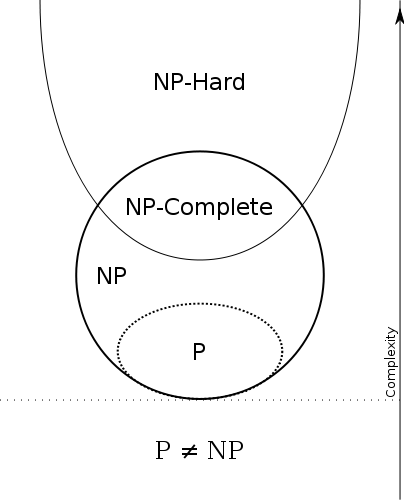
\includegraphics[scale=0.5]{images/complexity_classes.png}
	\caption{P κλάση και NP κλάση \\ πηγή: https://jcaip.github.io/Reduction-and-Intractibility/}
\end{matlab}

Το εντυπωσιακό στην περίπτωση των NP προβλημάτων είναι ότι πολλές φορές μπορεί να μοιάζουν εντυπωσιακά πολύ με κάποιο πρόβλημα που ανήκει στην κλάση P. Για παράδειγμα, δεδομένου ενός γράφου \(G = (V,E)\), η εύρεση ενός κύκλου Euler, δηλαδή ενός κύκλου που περνά από κάθε ακμή του γράφου ακριβώς μία φορά χωρίς να υπάρχει περιορισμός στο πλήθος των επισκέψεων ανά κόμβο έχει πολυπλοκότητα \(Ο(|Ε|)\). Να σημειώσουμε εδώ ότι ο παραπάνω κύκλος καλείται κύκλος Euler. Αντιθέτως, η εύρεση αν ένα γράφημα περιέχει κύκλο Hamilton, δηλαδή κύκλο που διέρχεται από κάθε κόμβο του γραφήματος ακριβώς μία φορά, είναι NP-πλήρες πρόβλημα. (Για περισσότερες πληροφορίες σχετικά με τα γραφήματα και τους κύκλους Hamilton μπορεί κανείς να ανατρέξει στην υποενότητα "Γραφήματα" της ενότητας "Μαθηματικό υπόβαθρο"). \\ 

\begin{mylemma}{TSP}{}
	Tο πρόβλημα του περιοδεύοντος πωλητή ανήκει στην κλάση NP.	
\end{mylemma}
 
Απόδειξη: \\
Για να αποδείξουμε ότι το TSP ανήκει στην κλάση NP αρκεί να βρούμε έναν αλγόριθμο, ο οποίος να επαληθεύει μία δεδομένη λύση σε πολυωνυμικό χρόνο. Έστω γράφημα \(G = (V,E)\) και \(k\) να είναι ένα threshold για την απόσταση που μπορεί να διανύσει ο πωλητής στην περίπτωση της βέλτιστης διαδρομής. Αν μία προτεινόμενη λύση είναι ένας κύκλος \(h\), τότε ο πολυωνυμικός αλγόριθμος που επαληθεύει μία λύση είναι ο παρακάτω. 

\begin{algorithm}[H]
	\SetAlgoLined
	\KwIn{Γράφημα \(G = (V,E)\), αριθμός \(k\) και κύκλος h}
	\KwResult{Απαντά ΝΑΙ στην περίπτωση που το h επαληθεύει λύση, αλλιώς απαντά ΟΧΙ}
	
	\If{h είναι Hamiltonian κύκλος του G}
	{
		sum = Υπολόγισε το άθροισμα των βαρών του h \;
		\If{sum \(\leq\) k}
		{
			Τύπωσε ΝΑΙ \;
		}
		\Else
		{
			Τύπωσε ΟΧΙ \;}
		}
	\Else
	{
		Τύπωσε ΟΧΙ \;
	}
	
	\caption{Επαλήθευση λύσης}
\end{algorithm}

Συνεπώς, το TSP είναι πρόβλημα που ανήκει στην κλάση NP. \\

Ένα σύνολο των προβλημάτων που ανήκουν στην κλάση NP καλούνται NP-complete και συγκροτούν ένα σύνολο προβλήματων NP. Πιο συγκεκριμένα, ένα πρόβλημα καλείται NP-complete αν ανήκει στην κλάση NP και κάθε άλλο πρόβλημα που ανήκει στην κλάση NP ανάγεται σε αυτό. Στο σημείο αυτό θα αποδείξουμε ότι το TSP είναι NP-complete. \\

\begin{mylemma}{TSP}{}
	Tο πρόβλημα του περιοδεύοντος πωλητή είναι NP-complete.	
\end{mylemma}

Απόδειξη: \\
Για να αποδείξουμε ότι το TSP είναι NP-complete πρέπει να αποδείξουμε ότι ανήκει στην κλάση NP και έπειτα να κάνουμε αναγωγή από ένα ήδη γνωστό NP-complete πρόβλημα. \\
Το πρώτο βήμα είναι εύκολο. Όπως αποδείχθηκε στο Λήμμα 4.0.1 το TSP ανήκει στην κλάση NP. \\
Για το δεύτερο βήμα επικαλούμαστε το πρόβλημα ύπαρξης κύκλου Hamilton σε ένα γράφημα, το οποίο είναι NP-complete. Θα ανάγουμε το πρόβλημα αυτό στο πρόβλημα του περιοδεύοντος πωλητή. \\
Έστω ότι έχουμε ένα στιγμιότυπο του προβλήματος εύρεσης κύκλου Hamilton και το γράφημα \(G = (V,E)\). Θα κατασκευάσουμε ένα καινούριο γράφημα \(G' = (V',E')\) όπου \(V' = V\) και \(E'\) θα περιλαμβάνει όλες τις δυνατές ακμές στο γράφημα. Κάθε ακμή στο \(G'\) θα έχει βάρος 1 αν είναι ακμή που υπήρχε και στο \(G\), αλλιώς θα έχει βάρος 2. Η κατασκευή ενός γραφήματος \(G'\) γίνεται σαρώνοντας το \(G\) και προσθέτοντας τις ακμές που λείπουν με κατάλληλα βάρη. Συνεπώς, η διαδικασία αυτή έχει πολυωνυμική πολυπλοκότητα. \\
Ως threshold της απόστασης του μονοπατιού που θα διανύσει ο πωλητής θέτουμε το \(|V|\). \\
Αν το \(G\) έχει Hamiltonian κύκλο, τότε και το \(G'\) θα έχει, αφού αποτελείται από τις ίδιες κορυφές και \(Ε \subseteq E'\). Ο κύκλος θα έχει άθροισμα βαρών ακμών ίσο με \(|V|\).
Αν το \(G'\) έχει Hamilton κύκλο με άθροισμα βαρών ακμών ίσο με \(|V|\), τότε ο κύκλος αυτός απαρτίζεται μόνο από τις κορυφές που έχουν βάρος 1, δηλαδή τις κορυφές που υπάρχουν και στο γράφημα \(G\). Συνεπώς, και το \(G\) έχει κύκλο Hamilton. \\
Συνεπώς, το TSP είναι NP-complete, γιατί είναι τόσο δύσκολο όσο το πρόβλημα ύπαρξης Hamilton κύκλου. \\

Στο σημείο αυτό κρίνεται σκόπιμο να αναφέρουμε ότι ο αποδοτικότερος τρόπος να μεταβεί κάποιος από ένα σημείο \(x\) σε ένα σημείο \(y\) είναι μεταβαίνοντας απευθείας στο \(y\) χωρίς ενδιάμεσους σταθμούς. Συνεπώς, η εξάλειψη των ενδιάμεσων σταθμών αποκλείεται να αυξήσει το κόστος της διαδρομής. Αυτό είναι μία ιδιότητα που αποτυπώνεται στην τριγωνική ανισότητα. 

\begin{align*}
	w(x,y) \leq w(x,z) + w(z,y)
\end{align*}

όπου \(w(x,y)\) το κόστος μετάβασης από το σημείο \(x\) στο σημείο \(y\). \\

Αν οι πόλεις που πρόκειται να επισκεφτεί ο πλανόδιος πωλητής είναι σημεία στο επίπεδο και η απόσταση μετράται με την Ευκλείδια απόσταση, τότε η τριγωνική ανισότητα ικανοποιείται και υπό αυτές τις συνθήκες το TSP είναι NP-complete, με άλλα λόγια δεν περιμένουμε αλγόριθμο που να επιλύει το πρόβλημα σε πολυωνυμικό χρόνο , αλλά κάποιον προσεγγιστικό αλγόριθμο. \\

Ένας προσεγγιστικός αλγόριθμος υπολογίζει σχεδόν βέλτιστες λύσεις και συνήθως αυτές αρκούν για τα NP-complete προβλήματα. Ένας προσεγγιστικός αλγόριθμος επιτυγχάνει λόγο προσέγγισης \(ρ(n)\), όπου \(n\) το μέγεθος της εισόδου του αλγορίθμου. Για τον \(ρ(n))\) ισχύει ότι

\begin{align*}
	\max\left(\frac{C}{C_{OPT}}, \frac{C_{OPT}}{C}\right) \leq ρ(n)
\end{align*}  

όπου \(C\) και \(C_{OPT}\) το κόστος της λύσης του προσεγγιστικού αλγορίθμου και της βέλτιστης λύσης αντίστοιχα. Ένας αλγόριθμος που επιτυγχάνει λόγο προσέγγισης \(ρ(n)\) καλείται \(ρ(n)\)-προσεγγιστικός. \\

\chapter{Μαθηματικό υπόβαθρο}

Η μελέτη σε βάθος του προβλήματος του περιοδεύοντος πωλητή χρήζει απαραίτητη την γνώση μερικών βασικών μαθηματικών εννοιών. Στο κεφάλαιο αυτό, παρουσιάζουμε και αναλύυμε, στον βαθμό που κρίνεται απαραίτητο, όλες τις μαθηματικές γνώσεις που χρειάζονται για την κατανοήση του TSP. \\

\section{Γραφήματα}

Βασική έννοια για τη μελέτη του προβήματος του περιοδέυοντος πωλητή είναι τα γραφήματα. Τα γραφήματα είναι ένα πολύ σημαντικά εργαλείο στα χερια των θεωρητικών πληροφορικών. Προσφέρουν πολλές διευκολύνσεις κατά τη μελέτη προβλημάτων (όπως και στην περίπτωση μας), είναι σχετικά απλά στη μελέτη και την κατανόηση τους και μπορούν εύκολα να κωδικοποιηθούν και να θεμελιωθούν με αυστηρό, μαθηματικό τρόπο. \\

\subsection{Βασική ορολογία}

Τα βασικά συστατικά ενός γραφήματος είναι  οι κορυφές και οι ακμές. Οι κορυφές ενώνονται με τη βοήθεια των ακμών και δημιουργούν ένα γράφημα. \\

Τα γραφήματα μπορούν να διακριθούν σε δύο βασικές κατηγορίες, τα κατευθυνόμενα γραφήματα και τη μη κατευθυνόμενα. \\

Ο αφηρημένος ορισμός στην περίπτωση των κατευθυνόμενων γραφημάτων περιλαμβάνει ένα διατεταγμένο ζεύγος \((V,E)\), όπου \(V\) είναι το σύνολο και το \(E\) είναι μία διμελής σχέση. Το \(V\) αποτελεί το σύνολο των κορυφών και το \(E\) το σύνολο των ακμών. Το κατευθυνόμενο γράφημα συμβολίζεται με \(G\). Ένα κατευθυνόμενο γράφημα μπορεί να αναπαρασταθεί γεωμετρικά ως ένα σύνολο από \(V\) σημεία, τα οποία ενώνονται με \(E\) βέλη. Ενα παραδειγμα γράφου φαίνεται στην εικόνα παρακάτω.

\begin{matlab}
	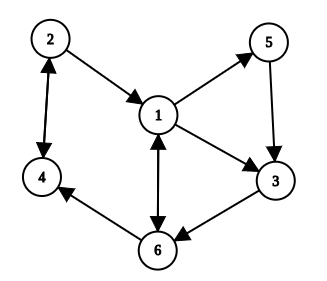
\includegraphics[scale=0.8]{images/directed_graph_example.png}
	\caption{Παράδειγμα κατευθυνόμενου γράφου \\ κατασκευάστηκε με: https://csacademy.com/app/graph\_editor/}
\end{matlab} 

Ο ορισμός για το μη κατευθυνόμενο γράφημα περιλαμβάνει ένα σύνολο \(V\) και ένα σύνολο πολυσυνόλων δύο στοιχείων \(E\). Το \(V\) αποτελεί και σε αυτήν την περιπτωση το σύνολο των κορυφών και το \(E\) το σύνολο των ακμών. Μία ενδεικτική γεμετρική αναπαράσταση δίνεται στην αντίστοιχη εικόνα παρακάτω. Και σε αυτήν την περίπτωση το \(V\) είναι ένα σύνολο σημείων, ωστόσο το \(E\) είναι ένα σύνολο γραμμών που δεν υποδικνύουν καμμία κατεύθυνση. \\

\begin{matlab}
	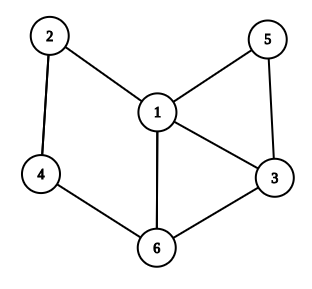
\includegraphics[scale=0.8]{images/undirected_graph_example.png}
	\caption{Παράδειγμα μη κατευθυνόμενου γράφου \\ κατασκευάστηκε με: https://csacademy.com/app/graph\_editor/}
\end{matlab}   

\subsection{Μονοπάτια}

Σε κάθε κατευθυνόμενο γράφημα οι ακμές περιέχουν μία αρχική κορυφή και μία τερματική κορυφή. Για παράδειγμα η ακμή (1,3) της εικόνας 3.1 περιέχει δύο κορυφές. Η κορυφή 1 καλείται αρχική κορυφή και η κορυφή 3 καλείται τερματική κορυφή. \\

Στα κατευθυνόμενα γραφήματα, μία ακολουθία ακμών \((e_1, e_2,...,e_k)\) όπου η τερματική κορυφή μίας ακμής \(e_j\) ταυτίζεται με την αρχική κορυφή της \(e_{(j+1)}\) καλείται μονοπάτι. \\

Αν ένα μονοπάτι δεν περιέχει την ίδια ακμή δύο φορές ονομάζεται απλό μονοπάτι. \\

Στοιχειώδες μονοποάτι καλείται το μονοπάτι εκείνο όπου δεν περιέχει την ίδια κορυφή παραπάνω από μία φορά. \\

Κύκλωμα καλείται το μονοπάτι \((e_1, e_2,...,e_k)\), όπου η τερματική κορυφή της \(e_k\) ακμής συμπίπτει με την αρχική κορυφή της \(e_1\) ακμής. \\

\subsection{Χαμιλτόνειοι κύκλοι και μονοπατια}

O Ιρλανδός φυσικός και μαθηματικός William Rowan Hamilton (4 Αυγούστου 1805 – 2 Σεπτεμβρίου 1865) μελέτησε εκτός των άλλων και τα γραφήματα. Συγκεκριμένα, δημιούργησε το μαθηματικό παιχνίδι "ο γύρος του κόσμου", του οποίου σκοπός ήταν η εύρεση ενός μονοπατιού από ακμές δωδεκαέδρου. Το μονοπάτι έπρεπε να περνά από κάθε κορυφή του δωδεκαέδρου ακριβώς μία φορά. Πιο συγκεκριμένα, ο ένας παίκτης κάρφωνε από μία βελόνα σε 5 διαδοχικές κορυφές και έπειτα ο άλλος παίκτης έπρεπε να συμπληρώσει το κύκλωμα έτσι ώστε να περιλαμβάνει όλες τις κορυφές. Μάλιστα, σε επιστολή προς τον φίλο του John T. Graves (17 Οκτωβρίου 1856) ο Hamilton τον πληροφορεί σχετικά με ένα παιχνίδι που βασίζεται στον εικοσιανό λογισμό (αλγεβρική δομή για τον υπολογισμών συμμετριών του εικοσαέδρου από τον ίδιο τον Hamilton) και την αναγνωρισιμότητα που έχει λάβει από μερικούς νεαρούς. Το παιχνίδι αυτό στάθηκε η αφορμή για την ανάπτυξη της θεωρίας γύρω από τα γραφήματα και προς τιμήν του Hamilton και του εν λόγω παιχνιδιού που επινόησε οι Χαμιλτονειανοί κύκλοι έλαβαν το όνομά του. \\

\begin{matlab}
	\includegraphics[scale=0.2]{images/Hamilton.png}
	\caption{William Rowan Hamilton \\ πηγή: https://en.wikipedia.org/wiki/William\_Rowan\_Hamilton}
\end{matlab}  

Η εύρεση ενός μονοπατιού ή ενός κυκλώματος που περνά από κάθε κορυφή ενός δεδομένου γραφήματος μόνο μία φορά φαντάζει αρχικά απλή υπόθεση, ωστόσο οι μέχρις στιγμής επιστημονικές προσεγγίσεις αποδεκνύουν το αντίθετο. 

Μονοπάτι (ή κύκλωμα) Hamilton είναι ένα μονοπάτι (ή ένα κύκλωμα) που περνά από όλες τις κορυφές ενός γραφήματος ακριβώς μία φορά. \\

Ένα γράφημα που περιέχει κύκλο Hamilton καλείται χαμιλτόνειο, ενώ αν δεν περιέχει καλείται μη χαμιλτόνειο. \\

Δυστυχώς, μέχρι και τώρα δε γνωρίζουμε κάποια ικανή και αναγκάια συνθήκη για την ύπαρξη μονοπατιών και κυκλωμάτων Hamilton. Δοθέντος ενός γραφήματος G, η απόδειξη ύπαρξης ή μη ενός μονοπατιού ή κυκλώματος Hamilton είναι η κατασκευή του. \\ 

\section{Delaunay Τριγωνοποίηση}

Στη υπολογιστική γεωμετρία, η τριγωνοποίηση πολυγώνων είναι ένα βασικό ζήτημα μελέτης. Με το όρο τριγωνοποίηση εννοούμε την διαμέριση της περιοχής που ορίζεται από το πολύγωνο σε τρίγωνα των οποίων η ένωση παράγει την περιοχή του αρχικού πολυγώνου. \\

Ουσιαστικά, η τριγωνοποίηση ενός συνόλου σημείων στο επίπεδο είναι ένα σύνολο τριγώνων. Η ένωση των τριγώνων αυτών ισούται με το κυρτό περίβλημα των σημείων και η τομή δύο τριγώνων μπορεί να είναι είτε κενή, είτε να είναι ίση με την κοινή κορυφή των δύο τριγώνων ή με την κοινή τους ακμή.

\begin{matlab}
	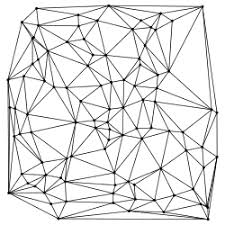
\includegraphics[scale=0.9]{images/delaunay_trianglulation.jpeg}
	\caption{Τριγωνοποίηση Delaunay \\ πηγή: https://en.wikipedia.org/wiki/Delaunay\_triangulation}
\end{matlab}

Στην παρούσα υποενότητα θα αναφερθούμε στη Delaunay τριγωνοποίηση, καθώς θα μας φανεί χρήσιμη στη μελέτη του προβλήματος του περιοδεύοντος πωλητή, με τρόπο που περιγράφεται σε επόμενη ενότητα. Επισημαίνουμε τη βασική θεωρία γύρω από την εν λόγω τριγωνοποίηση και μερικούς θεμελιώδεις αλγορίθμους που την παράγουν. \\

\subsection{Ιστορία}

Η delaunay τριγωνοποίηση ήταν μία επινόηση του Ρώσου μαθηματικού Boris Nikolaevich Delone. Ο Delone γεννήθηκε στις 15 Μαρτίου του 1890 και πέθανε έπειτα από 90 χρόνια, στις 17 Ιουλίου του 1980. Ο Boris Delone ασχολήθηκε με την άλγεβρα και τη γεωμετρία και μία από τις σημαντικότερες ανακαλύψεις του ήταν η τριγωνοποίηση Delaunay το 1934. \\

Η τριγωνοποίηση έλαβε το όνομα Delaunay, προς τιμήν του δημιουργού της, ο οποίος καλούσε τον εαυτό του "Boris Nikolaeviq Delone". Καθώς την εποχή εκείνη οι δύο επικρατέστερες γλώσσες στους επιστημονικούς κόλπους ήταν τα γαλλικά και τα γερμανικά, επικράτησε η γαλλική εκδοχή του ονόματός του και έτσι η τριγωνοποίηση έλαβε τελικά το όνομα Delaunay. \\

\begin{matlab}
	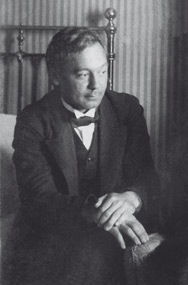
\includegraphics[scale=0.9]{images/Delone.jpg}
	\caption{Boris Nikolaevich Delone \\ πηγή: https://en.wikipedia.org/wiki/File:Delone\_cropped\_1924.jpg}
\end{matlab} 

\subsection{Βασική θεωρία}

Στόχος της τριγωνοποίησης Delaunay είναι με βάση ένα σύνολο σημείων στο επίπεδο να παράξει μία τριγωνοποίηση αυτών, η οποία να ικανοποιεί ορισμένες συνθήκες. \\

Για να μελετήσουμε την τριγωνοποίηση Delaunay πρέπει εξ αρχής να κάνουμε την παραδοχή ότι τα σημεία που πρόκειται να τριγωνοποιηθούν βρίσκονται σε γενική θέση. Γενική θέση στην παρούσα ενότητα εννοούμε ότι τέσσερα σημεία δε βρίσκονται πάνω στον ίδιο κύκλο.   \\

Αρχικά, εισάγουμε την απαραίτητη έννοια του "διανύσματος γωνιών" (vector angle). Έστω ότι \(P := \left\{ p_1, p_2,...,p_n \right\}\) είνα ένα σύνολο \(n\) σημείων στο επίπεδο. Επίσης, έστω ότι \(Τ\) είναι μια τριγωνοποίησή τους. Αν \(m\) είναι το σύνολο των τριγώνων που έχουν παραχθεί στη συγκεκριμένη τριγωνοποίηση, τότε με προφανή τρόπο εξάγεται το συμπέρασμα ότι το σύνολο των γωνιών που περιέχει η τριγωνοποίηση είναι \(3m\). Τοποθετούμε τις γωνίες της τριγωνοποίησης σε ένα διάνυσμα σε αύξουσα σειρά. Το διάνυσμα αυτό καλείται vector-angle και ορίζεται ως εξής

\begin{align}
	A(T) := (a_1, a_2, ..., a_{3m})
\end{align}   

όπου

\begin{align}
	a_i \leq a_j \text{, } \forall i<j
\end{align}

Αν \(Τ'\) είναι μια διαφορετική τριγωνοποίηση από την \(Τ\) για το ίδιο σύνολο σημείων \(P\) και το αντίστοιχο διάνυσμα γωνιών είναι το \(A(T') = (a_{1}', a_{2}', ..., a_{3m}')\), θα λέμε ότι το διάνυσμα γωνιών της \(Τ\) τριγωνοποίησης είναι μεγαλύτερο από το διάνυσμα γωνιών της \(Τ'\) τριγωνοποίησης και θα γράφουμε \(Α(Τ) > Α(Τ')\) αν υπάρχει \(i\), όπου \(1 \leq i \leq 3m\) τέτοιο ώστε 

\begin{align*}
	a_j = a_{j}' \text{, } \forall j < i \text{ και } a_i > a_{i}'
\end{align*}

Θα δούμε στη συνέχεια ότι στόχος μας εδώ είναι να καταφέρουμε να εντοπίσουμε το μεγαλύτερο διάνυσμα γωνιών. \\

Θα λέμε ότι μία τριγωνοποίηση είναι "angle-optimal" και θα γράφουμε \(Α(Τ) \geq A(T')\) αν \(Α(Τ) > Α(Τ')\) για όλες τις δυνατές τριγωνοποιήσεις \(T'\). \\

Στο σημείο αυτό πρέπει να αναφέρουμε ότι το πλήθος των τριγώνων που προκύπτουν από μία τριγωνοποίηση δεν είναι τυχαίο. Μπορεί να καθοριστεί με ακρίβεια, πράγμα που ήδη έχει διατυπωθεί σε αντίστοιχο θεώρημα. \\

\begin{mytheorem}{Πλήθος ακμών και τριγώνων τριγωνοποίησης σημείων στο επίπεδο}{Α}
	Έστω \(P\) ένα σύνολο \(n\) σημείων στο επίπεδο. Έστω ότι τα σημεία δεν είναι όλα μεταξύ τους συνευθειακά και έστω με \(k\) να συμβολίζονται ότα τα σημεία που βρίσκονται στο όριο του convex hull του \(P\). Οποιαδήποτε τριγωνοποίηση των σημείων του \(P\) παράγει \(2n - 2 - k \) τρίγωνα και \(3n - 3 - k\) ακμές.
\end{mytheorem}

Απόδειξη: \\
Έστω ότι τα \(P\) σημεία τριγωνοποιούνται και παράγονται \(m\) το πλήθος τρίγωνα. Συνεπώς, το επίπεδο έχει διαχωριστεί με \(m + 1\) υποπεριοχές. \\
Κάθε τρίγωνο έχει 3 ακμές και το convex hull έχει \(k\) ακμές. \\
Κάθε ακμή ανήκει σε δύο υποπεριοχές του επιπέδου. \\
Συνεπώς, ο συνολικός αριθμός ακμών είναι  \(\frac{3m + k}{2}\). \\
Από τον τύπο του Euler, όπου \(n_f = m + 1\) και \(n_e = \frac{3m + k}{2}\), προκύπτει ότι 

\begin{align*}
	n - n_e + n_f= 2 & \Leftrightarrow \\
	n - \frac{3m + k}{2} + (m+1) = 2 & \Leftrightarrow \\	
	2n - (3m + k) + 2(m+1) = 4 & \Leftrightarrow \\
	2n - 3m - k + 2m + 2 = 4 & \Leftrightarrow \\
	2n - m - k = 2 & \Leftrightarrow \\
	m = 2n - k - 2
\end{align*}

και αφού \(m = 2n - 2 - k\), το \(n_e\) υπολογίζεται να είναι

\begin{align*}
	n_e = \frac{3m + k}{2} & \Leftrightarrow \\
	n_e = \frac{3(2n - k - 2) + k}{2} & \Leftrightarrow \\
	n_e = \frac{6n - 3k - 6 + k}{2} & \Leftrightarrow \\
	n_e = \frac{6n - 6 - 2k}{2} & \Leftrightarrow \\
	n_e = 3n - 3 - k
\end{align*}

\(\square \)

Όπως ήδη αναφέραμε στόχος είναι να βρεθεί η τριγωνοποίηση που δίνει το "μεγαλύτερο" διάνυσμα γωνιών. Για να καταφέρουμε να φτάσουμε στο σημείο να παράξουμε μία τέτοια τριγωνοποίηση για ένα δεδομένο σύνολο σημείων πρέπει να αναφέρουμε μερικές ακόμα θεμελιώδεις έννοιες. Εισάγουμε την έννοια της "παράνομης ακμής" (illegal edge). \\

Έστω μία τριγωνοποίηση των \(P\) σημείων και έστω μία ακμή της τριγωνοποίησης που βρίσκεται εντός ενός κυρτού τετράπλευρου και είναι κοινή ακμή για δύο διαφορετικά τρίγωνα της τριγωνοποίησης. Η ακμή αυτή μπορέι να γίνει flip. Στην περίπτωση αυτή το μόνο που αλλάζει είναι το \(A(T)\). \\

\begin{mydefinition}{Παράνομη ακμή}{α}
	Έστω \(T\) μία τριγωνοποίηση των σημείων \(P\).  Καλούμε μία ακμή "παράνομη" εαν μπορούμε να αυξήσουμε τη μικρότερη γωνία του διανύσματος γωνιών κάνοντάς την flip.
\end{mydefinition}

Αν \(T\) μία τριγωνοποίηση που περιέχει μία παράνομη ακμή και \(T'\) η τριγωνοποίηση που έχει γίνει flip η παράνομη ακμή, τότε ισχύει ότι η \(T'\) είναι angle-optimal:

\begin{align*}
	A(T') \geq A(T)
\end{align*}

\begin{mydefinition}{}{}
	Μία τριγωνοποίηση \(T\) καλείται νόμιμη εαν δεν περιέχει καμία παράνομη ακμή.
\end{mydefinition}

Συνεπώς, κάθε angle-optimal τριγωνοποίηση είναι νόμιμη. \\

Με βάση αυτήν την τεχνική μπορούμε να οδηγηθούμε σε μία τριγωνοποίηση Delaunay. \\

\begin{mydefinition}{Τριγωνοποίηση Delaunay}{}
	Για ένα σύνολο σημείων \(P\) στο επίπεδο, η τριγωνοποίηση Delaunay είναι η τριγωνοποίηση εκείνη που δεν περιέχει καμία παράνομη ακμή. Συμβολίζουμε την τριγωνοποίηση Delaunay των σημείων με \(Del(P)\).
\end{mydefinition}

Μία εναλλακτική προσέγγιση των flips και των ελέγχων των διανυσμάτων γωνιών για την παραγωγή Delaunay τριγωνοποίησης είναι η προσέγγιση με τη βασικό εργαλείο τον κύκλο. Στο σημείο αυτό, επισημαίνουμε κάποιες βασικές ιδιότητες που αφορούν τον κύκλο και πηγάζουν από το θεώρημα του Θαλή. \\

\begin{matlab}
	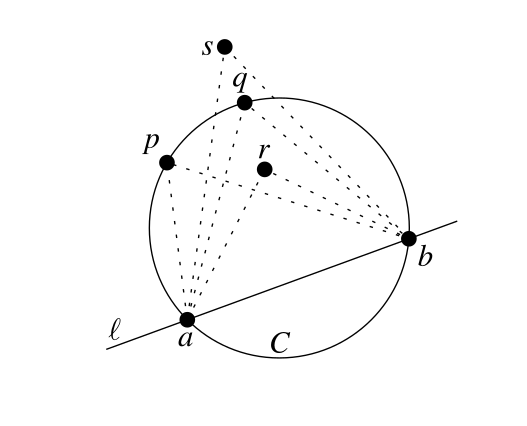
\includegraphics[scale=0.4]{images/circle.png}
	\caption{Κύκλος C με τόξο ab \\ πηγή: "Computational Geometry, Algorithms and Applications,Third Edition", σελ. 194}
\end{matlab}

\begin{mytheorem}{Γωνίες που βαίνουν σε χορδή}{χορδη1}
	Έστω \(C\) να είναι ένας κύκλος και \(l\) μία ευθεία που τέμνει τον κύκλο στα σημεία \(a\) και \(b\). Έστω \(p\) και \(q\) σημεία πάνω στην περίμετρο του κύκλου. Τότε η γωνία που βαίνει στο τόξο \(ab\) με κορυφή το σημείο \(p\) είναι ίση με την γωνία που βαίνει στο ίδιο τόξο και έχει κορυφή το σημείο \(q\). 
\end{mytheorem}

\begin{mytheorem}{Γωνίες που βαίνουν σε χορδή}{χορδη2}
	Έστω \(C\) να είναι ένας κύκλος και \(l\) μία ευθεία που τέμνει τον κύκλο στα σημεία \(a\) και \(b\). Έστω \(r\) ένα σημείο εντός του κύκλου και \(s\) ένα σημείο εκτός. Τότε η γωνία που βαίνει στο τόξο \(ab\) με κορυφή το σημείο \(r\) είναι μεγαλύτερη από την γωνία που βαίνει στο ίδιο τόξο και έχει κορυφή το σημείο \(s\). 
\end{mytheorem}

Συνοψίζοντας 

\begin{align}
	\angle arb > \angle apb = \angle aqb > \angle asb
\end{align}

Από όλα τα παραπάνω προκύπτει ότι \\

\begin{mylemma}{}{}
	Έστω \(C\) ένας κύκλος και \(p_i, p_j, p_k\) σημεία πάνω στον κύκλο και \(p_l\) σημείο εντός του κύκλου. Αν τα \(p_i, p_j, p_k, p_l\) σχηματίζουν ένα κυρτό πολύγωνο, τότε αυτό μπορεί να τριγωνοποιηθεί και να παραχθούν τα τρίγωνα \(p_i p_j p_k\) και \(p_i p_j p_l\) με κοινή ακμή την \(p_i p_j\). Η ακμή \(p_i p_j\) είναι παράνομη.
\end{mylemma} 

\begin{mylemma}{}{}
	Έστω \(C\) ένας κύκλος και \(p_i, p_j, p_k\) σημεία πάνω στον κύκλο και \(p_l\) σημείο εκτός του κύκλου. Αν τα \(p_i, p_j, p_k, p_l\) σχηματίζουν ένα κυρτό πολύγωνο, τότε αυτό μπορεί να τριγωνοποιηθεί και να παραχθούν τα τρίγωνα \(p_i p_j p_k\) και \(p_i p_j p_l\) με κοινή ακμή την \(p_i p_j\). Η ακμή \(p_i p_j\) είναι νόμιμη.
\end{mylemma} 

Φυσικά, να υπενθυμίσουμε ότι τα σημεία βρίσκονται σε γενική θέση, συνεπώς δεν παίρνουμε την περίπτωση τα \(p_i, p_j, p_k, p_l\) να είναι και τα 4 πάνω στον ίδιο κύκλο. \\

Στο παραακάτω θεώρημα συνοψίζεται η προσέγγιση της τριγωνοποίησης με εργαλείο τον κύκλο. \\

\begin{mytheorem}{Η ιδιότητα των κενών κυκλων}{}
	Έστω \(P\) ένα σύνολο σημείων στο επίπεδο που βρίσκονται σε γενική θέση. Μία τριγωνοποίηση \(T\) είναι τριγωνοποίηση Delaunay αν και μόνο αν ο κυκλος που σχηματίζεται από κάθε τριάδα σημείων που αποτελούν τρίγωνο της τριγωνοποίησης δεν περιέχει κανένα άλλο σημείο του \(P\) στο εσωτερικό του.
\end{mytheorem} 

Απόδειξη: \\
\(\Rightarrow \) \\
Αν κανένα σημείο του συνόλου σημείων \(P\) δεν βρίσκεται εσωτερικά του εκάστοτε κύκλου που σχηματίζεται από τις τρεις κορυφές ενός τριγώνου της τριγωνοποίησης, τότε όλες οι ακμές είναι νόμιμες. Συνεπώς, η τριγωνοποίηση είναι νόμιμη. \\
\(\Leftarrow \) "Αν μια τριγωνοποίηση είναι Delaunay, τότε κανένα σημείο του \(P\) δεν βρίσκεται εντός του εκάστοτε κύκλου τριών κορυφών τριγώνου της τιγωνοποίησης" \\
Θα αποδείξουμε αυτήν την κατεύθυνση με απαγωγή σε άτοπο. \\
Έστω ότι η τριγωνοποίηση \(T\) είναι τριγωνοποίηση Delaunay και έστω ότι υπάρχει κύκλος που περιέχει σημεία του \(P\) εκτός των \(A, B, C\) που τον ορίζουν και είναι οι κορυφές ενός τριγώνου της τριγωνοποίησης. \\
Έστω ότι από όλα αυτά τα σημεία επιλέγεται εκείνο που απέχει την μικότερη απόσταση απο την ακμή του τριγώνου, έστω \(D\). \\
Επειδή η τριγωνοποίηση είναι Delaunay, το τρίγωνο \(BCD\) δε μπορεί να ανήκει στην τριγωνοποίηση. \\
Έστω \(Ε\) ένα σημείο εκτός του κύκλου και \(BCE\) τρίγωνο. Το \(D\) βρίσκεται εντός του κύκλου που ορίζεται από τα σημεία \(B, C, E\) και εκτός του τριγώνου \(BCE\). 
......................................

\begin{matlab}
	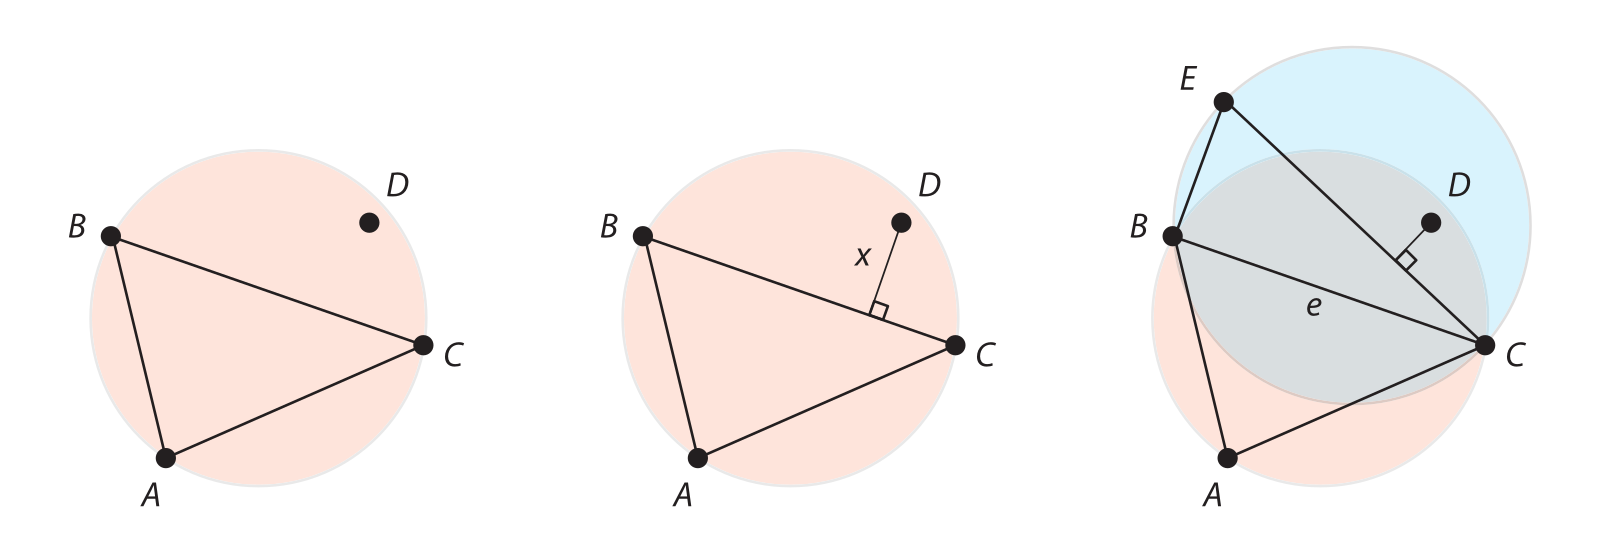
\includegraphics[scale=0.3]{images/emptycircle.png}
	\caption{Απόδειξη του θεωρήματος 3.2.4 \\ πηγή: "Discrete and Computational Geometry", σελ.: 86}
\end{matlab} 

Συνοψίζουμε τα κριτήρια για την Delaunay τριγωνοποίηση σε ένα θεώρημα. \\

\begin{mytheorem}{Delaunay Τριγωνοποίηση}{}
	Σε μία τριγωνοποίηση Delaunay \(T\) των σημείων \(P\): \\
	1. Τρία σημεία κατασκευάζουν τρίγωνο αν και μόνο αν ο περιγεγραμμένος ανοιχτός κύκλος του δεν περιέχει κανένα άλλο σημείο του \(P\). \\
	2. Δύο σημεία κατασκευάζουν ακμή αν και μόνο αν υπάρχει κύκλος με τα σημεία αυτά στην περιφέρειά του που δεν περιέχει κανένα άλλο σημείο του \(P\) 	
\end{mytheorem}

Για δεδομένη τριγωνοποίηση, θα αποφασίζουμε αν αυτή είναι Delaunay ανν ο περιγεγραμμένος κύκλος κάθε τριγώνου δεν περιέχει κανένα άλλο σημείο. \\

\subsection{Κατασκευή Delaunay Τριγωνοποίησης}

Αφού είδαμε τη θεωρητική βάση της τριγωνοποίησης Delaunay, μπορούμε πλέον να αναφερθούμε σε τεχνικές και αλγόριθμους που κατασκευάζουν μία τριγωνοποίηση Delaunay. \\

\subsubsection{Αυξητκός αλγόριθμος}

Ο αλγόριθμος αυτός δε γνωρίζει εκ των προτέρων όλα τα σημεία που πρόκειται να τριγωνοποιηθούν. Για τη ακρίβεια, λαμβάνει ένα σύνολο σημείων, σε κάθε βήμα του εξετάζει ενα απο τα σημεία αυτά και παράγει την τρέχουσα Delaunay τριγωνοποίηση σαν να μην υπάρχουν άλλα σημεία προς εξέταση, μέχρι που εξετάζει όλο το σύνολο σημείων και παράγει της τελική Delaunay τριγωνοποίηση. Η επιλογή σημείου σε κάθε βήμα γίνεται με τυχαίο τρόπο. \\

Ο αλγόριθμος έχει \(Ο(n logn)\) μέση πολυπλοκότητα, ενώ στη χείριστη περίπτωση η πολυπλοκότητά του είναι \(O(n^2)\). \\

Ο αλγόριθμος επιλέγει 3 σημεία στο επίπεδο των οποίων το αντίστοιχο τρίγωνο περιλαμβάνει όλα τα σημεία προς τριγωνοποίηση. Η επιλογή των τριών αυτών σημείων δεν είναι τυχαία και πρέπει να πληρεί ορισμένα κριτήρια. Θα αναφερθούμε σε αυτά στη συνέχεια, αφού πρώτα παρουσιάσουμε τον πυρήνα του αλγορίθμου. \\

Ο αλγόριθμος αυξητικά παράξει σε κάθε του βήμα την τριγωνοποίηση. Για κάθε σημείο που ελέγχει εντόπίζει αν βρίσκεται εντός τριγώνου της ήδη κατασκευασμένης τριγωνοποίησης ή πάνω σε κάποια ακμής της τριγωνοποίησης. Στην περίπτωση που βρίσκεται μέσα σε τρίγωνο κατασκευάζονται τρείς νέες ακμές, οι οποίες εκτείνονται από το υπό εξέταση σημείο προς την κάθε κορυφή του τριγώνου που το περιέχει. Στην περίπτωση που το σημείο βρίσκεται πάνω σε ακμή της τριγωνοποίησης είναι εύκολο κανείς να συνειδητοποιήσει ότι η ακμή αυτή είναι κοινή ακμή για δύο τριγωνα. Συνεπώς, δημιουργούνται δύο νέες ακμές από το σημείο που εξετάζεται προς τη μία κορυφη του ενός και του άλλου τριγώνου που δεν ανήκουν στο ευθύγραμμο τμήμα. Για την καλύτερη κατανόηση των δύο περιπτώσεων παρέχεται η αντίστοιχη εικόνα. Αφού δημιουργηθούν οι νέες ακμές με κατάλληλο τρόπο μένει να ελέγξουμε ότι η τριγωνοποίηση που έχει παραχθεί είναι Delaunay. Η προσθήκη μιας νέας ακμής μπορεί να κάνει παράνομες τις ήδη υπάρχουσες ακμές της τριγωνοποίησης. Αυτο αντιμετωπίζεται με κατάλληλα flips κάθε φορά. Ο αλγόριθμος παρουσιάζεται συνοπτικά παρακάτω. \\

Ο αλγόριθμος σαφώς τερματίζει, καθώς το πλήθος των ακμών της τριγωνοποίησης είναι πεπερασμένο. Επίσης, ο αλγόριθμος είναι ορθός διότι εξετάζει κάθε ακμή ως προς την "νομιμότητά" της στο βήμα όπου καλεί τον αλγόριθμο "Νομιμοποίηση ακμής". Συνεπώς, ποτέ δε θα προκύψει παράνομη ακμή χωρίς να ελεγχθεί και να μετατραπεί σε νόμιμη. όπως ήδη έχουμε αναφέρει, μια τριγωνοποίηση είναι Delaunay αν είναι νόμιμη. \\

\begin{algorithm}[H]
	\SetAlgoLined
	\KwIn{n σημεία του επιπέδου}
	\KwResult{Τριγωνοποίηση Delaunay για n σημεία του επιπέδου}
	
	Δημιούργησε κατάλληλα σημεία \(p_{-1}, p_{-2}, p_{-3}\) στο επίπεδο έτσι ώστε το τρίγωνο που σχηματίζουν να περέχει τα n σημεία εισόδου. \;
	\For{ένα σημείο του επιπέδου που δεν έχει ενταχθέι στην τριγωνοποίηση}
	{Βρες σε ποιο τρίγωνο ή ακμή ανήκει \;
	\If{σημείο ανήκει σε τρίγωνο}
		{Πρόσθεσε 3 νέες ακμές προς τις κορυφές του τριγώνου \;
		Κάλεσε τον αλγόριθμο 2 για τις 3 πλευρές του τριγώνου \;}
	\Else
		{Πρόσθεσε 2 νέες ακμές προς τις κορυφές των τριγώνων που έχουν κοινή πλευρά την πλευρά που ανήκει το υπο εξέταση σημείο \;
		Κάλεσε τον αλγόριθμο 2 για τις 4 πλευρές των 2 τριγώνων \;}
	}	
	
	\caption{Αυξητικός αλγόριθμος τριγωνοποίησης Delaunay}
\end{algorithm}

\begin{algorithm}[H]
	\SetAlgoLined
	\KwIn{Τριγωνοποίηση σημείων, ακμή της τριγωνοποίησης \(p_i p_j\), σημείο \(p_r\)}
	\KwResult{Τριγωνοποίηση που είναι νόμιμη}
	
	Βρές τρίγωνο \((p_i, p_j, p_l)\) \;
	\If{\(p_i p_j\) παράνομη}
	{Διαγραφή \(p_i p_j\) \;
	Δημιουργία \(p_r p_l\) \;
	\(p_i p_l\) = νόμιμη ως προς την \(p_r\) \;
	\(p_j p_l\) = νόμιμη ως προς την \(p_r\) \;}
	
	\caption{Νομιμοποίηση ακμής}
\end{algorithm}

\begin{matlab}
	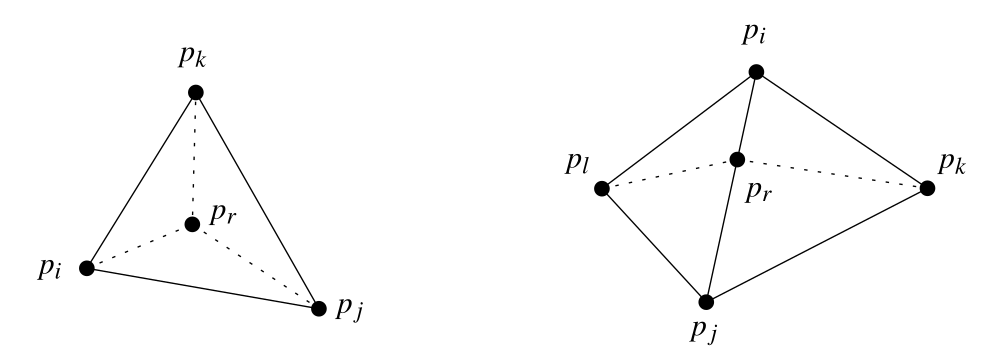
\includegraphics[scale=0.3]{images/incremental.png}
	\caption{Οι δύο περιπτώσεις που εξετάζει ο αυξητικός αλγόριθμος κατά την εισαγωγή ενός νέου σημείου \(p_r\). Αριστερά φαίνεται η πρώτη περίπτωση, όπου το νεό σημείο εντοπίζεται εντός τριγώνου της τριγωνοποίησης, ενώ δεξία φαίνεται η δεύτερη περίπτωση όπου το νέο σημείο βρίσκεται πάνω σε ακμή της τριγωνοποίησης \\ πηγή: "Computational Geometry, Algorithms and Applications, Third Edition", σελ.: 200}
\end{matlab} 

Στο σημείο αυτό μπορούμε να εξηγήσουμε τον τρόπο που επιλέγουμε τα τρία αρχικά σημεία που δημιουργούν τρίγωνο που περιβάλει όλα τα προς τριγωνοποίηση σημεία. Ουσιαστικά, τα σημεία αυτά πρέπει να λάβουν θέσεις στο επίπεδο, που να μην επηρεάζουν την έκβαση της τριγωνοποίσης μετέπειτα. Αυτό επιτυγχάνεται μόνο αν τοποθετηθούν αρκετά μακρυά από τα σημεία που πρόκειται να τριγωνοποιηθούν. Για να συμβεί αυτό πρέπει καθένα από τα σημεία \(p_{-1}, p_{-2}, p_{-3}\) να μην βρίσκονται εντός των κύκλων που σχηματίζονται από όλες τις δυνατές τριάδες σημειων. Μόνο τότε μπορούμε να είμαστε βέβαιοι ότι δεν έχουν επηρεάσει την τριγωνοποίηση Delaunay. \\

Τέλος, πρέπει να αποσαφηνίσουμε τον τρόπο με τον οποίον ο αλγόριθμος αντιλαμβάνεται πότε ένα σημείο είναι εντός τριγώνου ή πάνω σε κάποια ακμή. Αυτό επιτυγχάνεται με τη δημιουργία ενός κατάλληλου κατευθυνόμενου ακυκλικού γράφου. Ο γράφος αυτός κωδικοποιεί όλα τα τρίγωνα που δημιουγήθηκαν κατά την εκτέλεση του αλγορίθμου και την χρονική τους ιεραρχία. Οι κόμβοι είναι τρίγωνα και οι ακμές δηλώνουν τις σχέσεις μεταξύ δύο τριγώνων. Αν δύο κόμβοι συνδέονται με ακμή, δηλαδη με σχέση "πατέρα - παιδιού", τότε τα αντίστοιχα τρίγωνα έχουν μη κενή τομή. Είναι προφανές πως η ρίζα του γράφου είναι το τρίγωνο \(p_{-1} p_{-2} p_{-3}\). Έχουμε ήδη αναφέρει ότι η προσθήκη ενός νέου σημείου μπορεί να δημιουργήσει τρία ή τέσσερα τρίγωνα στην τριγωνοποίηση. Σε όρους γράφου, αυτό σημαίνει τρία ή τέσσερα νέα φύλλα. Το flip μιας ακμής δημιουργεί μόνο δύο φύλλα. \\

Για τον εντοπισμό ενός σημείου, διατρέχεται ο γράφος ξεκινόντας από τη ρίζα. Ελέγχονται τα τρία παιδία της ρίζας και εντοπίζουμε σε ποιο από αυτά τα τρία τρίγωνα (που περιέχονται στους κόμβους) ανήκει το προς εξέταση σημείο. Μεταβαίνουμε στο κατάλληλο παιδί και συνεχίζουμε την ίδια ακριβώς διαδικασία μέχρι να φτάσουμε σε φύλλο του γράφου στο οποίο και εντοπίζεται το σημείο που εξετάζουμε. \\ 

\chapter{Γραφοθεωρητική Προσέγγιση του Προβλήματος του πλανόδιου πωλητή}
 
Η προσέγγιση του TSP με βάση τη θεωρία γραφημάτων συνδέεται στενά με τα τους Χαμιλτόνειους κύκλους. Επί της ουσίας το πρόβλημα του περιοδεύονοτς πωλητή είναι μία επέκταση του προβλήματος εύρεσης κυκλώματος Hamilton. \\ 

Όπως ήδη έχουμε αναφέρει στην εισαγωγή, στόχος του προβλήματος είναι ο πωλητής να επισκεφτεί ένα σύνολο πόλεων, ακριβώς μία φορά την κάθε μία, ελαχιστοποιόντας τις αποστάσεις που πρέπει να διανύσει. Αν αναπαραστήσουμε το σύνολο των πόλεων προς επίσκεψη με ένα σύνολο κορυφών \(V\) και το σύνολο όλων των πιθανών διαδρομών με ενα σύνολο \(E\), τότε μπορούμε να μεταφέρουμε την εικόνα του χάρτη που μελετά ο πωλητής σε γραφική αναπαράσταση. Ο πωλητής εκκινεί και τερματίζει το ταξίδι του στην ίδια πόλη και επισκέπτεται όλες τις υπόλοιπες ακριβώς μία φορά, διανύοντας το έλαχιστον συνολικό μήκος. \\

Θεωρούμε το παραπάνω γράφημα του χαρτη των πόλεων και των αντίστοιχων διαδρομών να είναι το \(G = (V,E,w(i,j))\), όπου το \(V\) περιλμβάνει τις \(n\) πόλεις  (κορυφές), το \(E\) τις διαδρομές μεταξύ δύο πόλεων (ακμές) και το \(w\) να είναι μία συνάρτηση 

\begin{align}
	w:E \rightarrow \R^{+}
\end{align} 
 
τέτοια ώστε να ισχύει 

\begin{align}
	w(i,k) \leq w(i,j) + w(j,k)
\end{align} 

Ουσιαστικά το \(w(i,j)\) είναι το μήκος της διαδρομής από την πόλη \(i\) στην πόλη \(j\) ή με όρους γραφημάτων το βάρος της ακμής \((i,j)\). Στην περίπτωση κυκλώματος, το μήκος του ορίζεται να είναι το άθροισμα των μηκών των αντίστοιχν ακμών. \\

Το TSP αναζητά ένα κύκλωμα Hamilton με ελάχιστο μήκος. Δυστυχώς, μέχρι και σήμερα δε γνωρίζουμε κανέναν αλγόριθμο που να επιλύει το πρόβλημα του περιοδεύοντος πωλητή για μερικές εκατοντάδες πόλεων σε εύλογα χρονικά πλαίσια. \\

\section{Η μέθοδος του πλησιέστερου γείτονα}

Μία πολύ απλή μέθοδος για την εύρεση Χαμιλτονειανού κύκλου σε ένα γράφημα \(G = (V,E,w(i,j))\) είναι η μέθοδος του πλησιέστερου γείτονα. 

\begin{algorithm}[H]
	\SetAlgoLined
	\KwResult{Κύκλωμα Hamilton για το πρόβλημα του περιοδέυοντος πωλητή}
	
	Επέλεξε αυθαίρετα μία κορυφή v \;
	Ανέθεσε την v στην x \;
	\For{x} 
	{Επέλεξε μία κορυφή v που δεν βρίσκεται στο μονοπάτι και απέχει τη μικρότερη απόσταση από την τρέχουσα x \;
	Πρόσθεσε την ακμή (x,v) στο μονοπάτι \;
	Ανανέωσε την x με την v \;}
	Σχημάτισε κύκλωμα συνδέοντας την αρχική κορυφή με την τελική κορυφή του μονοπατιού \;
	
	\caption{Μέθοδος πλησιέστερου γείτονα}
\end{algorithm}

\chapter{Γεωμετρική Προσέγγιση του Προβλήματος του πλανόδιου πωλητή}

\section{Προσέγγιση με βάση την τριγωνοποίηση Delaunay}

Ένας από τους πλέον διαδεδομένους γεωμετρικούς τρόπους προσέγγισης του προβλήματος του περιοδεύοντος πωλητή είναι η προσέγγιση με βάση την τριγωνοποίσηση Delaunay. Έχουμε αναφερθεί εκτενώς στην τριγωνοποίηση Delaunay στο αντίστοιχο κεφάλαιο που αφορά το απαραίτητο μαθηματικό υπόβαθρο για την κατανόηση της παρούσας μελέτης. \\

Η τριγωνοποίηση Delaunay έχει μερικά χαρακτηριστικά τα οποία μπορούν να φανούν ιδιαιτέρως σημαντικά στο πρόβλημα του πλανόδιου πωλητή. 

\begin{itemize}
	\item Μεγιστοποιεί τη μικρότερη γωνία των τριγώνων της τριγωνοποίησης.
	\item Μπορεί να υπολογιστεί σε χρόνο \(Ο(n \log(n))\).
	\item Για κάθε τρίγωνο της τριγωνοποίησης υπάρχει κύκλος που περιέχει τις τρεις κορυφές του τριγώνου και μόνο αυτές.
	\item Είναι μοναδική αν δεν υπάρχουν τέσσερα σημεία που βρίσκονται στον ίδιο κύκλο.
	\item Περιέχει proximity graphs όπως το MST, το nearest neighbor graph, relative neighbor graph, Gabriel graph.
\end{itemize}

Η Delaunay τριγωνοποίηση μπορεί να συμβάλλει στην εύρεση μιας κατάλληλης διαδρομής για τον πλανόδιο πωλητή. Ωστόσο, δεν είναι απαραίτητο ότι θα καταφέρει να εντοπίσει την βέλτιστη διαδρομή, δηλαδή τη διαδρομή εκείνη που ελαχιστοποιεί το συνολικό κόστος, με άλλα λόγια τη συνολική απόσταση που χρειάζεται να διανύσει ο πωλητής. Υπάρχουν περιπτώσεις, όπου οι αλγόριθμοι επίλυσης του TSP με τη βοήθεια της Delaunay τριγωνοποίησης δεν παράγουν το βέλτιστο μονοπάτι. Το βέλτιστο μονοπάτι δεν είναι πάντοτε ένα υποσύνολο του Delaunay γράφου. Ένα τέτοιο παράδειγμα φαίνεται στην εικόνα 5.1. Ωστόσο, η Delaunay τριγωνοποίηση μπορεί να δώσει μία αρκετά καλή προσέγγιση της λύσης του προβλήματος. \\

Στην υποενότητα αυτή παρουσιάζουμε έναν αλγόριθμο εύρεσης μονοπατιού για το πρόβλημα του πλανόδιου πωλητή με βάση την Delaunay τριγωνοποίηση όπως παρουσιάζεται στο \cite{10}. \\

\begin{matlab}
	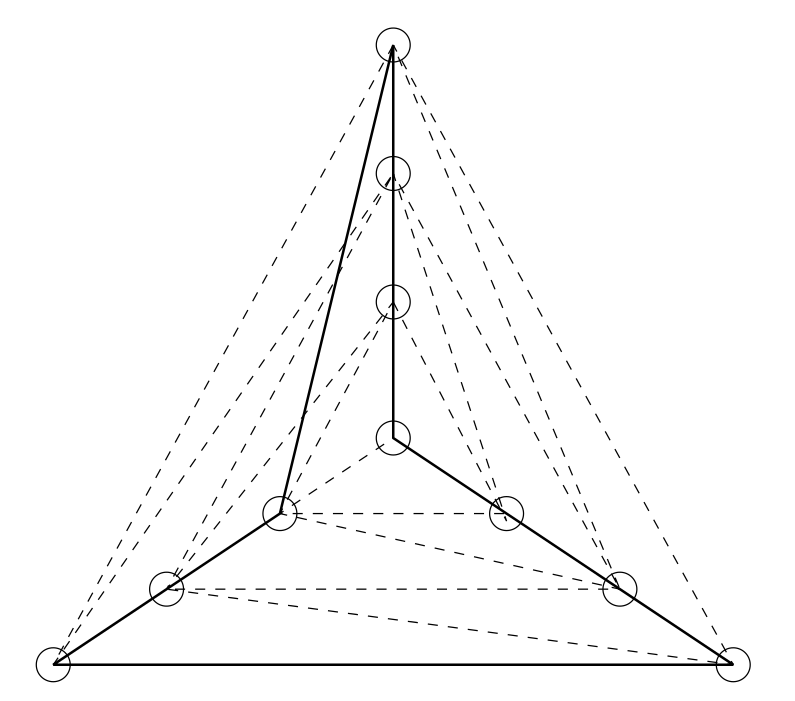
\includegraphics[scale=0.5]{images/delaunay_optimum_tour.png}
	\caption{Η καλύτερη διαδρομή δεν είναι στο υποσύνολο του Delaunay γράφου \\ πηγή: "An O(n log n) Heuristic for the Euclidean Traveling Salesman Problem" \cite{10} }
\end{matlab} 

Πρωτού ξεκινήσει η διαδικασία κατασκευής της διαδρομής, οι πόλεις, που πλέον λογίζονται ως σημεία στο επίπεδο, πρέπει να έχουν περάσει από τη διαδικασία της τριγωνοποίησης Delaunay. Έπειτα, από την τριγωνοποίηση των σημείων ο αλγόριθμος έχει να διαχείριστεί έναν γράφο, όπου οι πόλεις είναι οι κόμβοι του γράφου και οι διαδρομές (οι ακμές που έχουν παραχθεί από την τριγωνοποίηση) είναι οι ακμές του γράφου. Ο αλγόριθμος ξεκινά με μία διαδρομή \(T_i\) που περιέχει κάποιες από τις πόλεις σταθμούς και \(i\) το πλήθος ακμές που υποδεικνυουν την διαδρομή. Επιχειρεί με επαναλαμβανόμενα βήματα να εντάξει και τις υπόλοιπες. \\

Στο σημείο αυτό αναφέρουμε τον απαραίτητο συμβολισμό για την περαιτέρω ανάλυση του αλγορίθμου. \\

\begin{align*}
	& \bullet \text{ } E_{mn} \text{ είναι η ακμή που συνδέει τις πόλεις } C_m, C_n \\
	& \bullet \text{ } C_L(E_{mn}) \text{ είναι η πόλη που βρίσκεται στο αριστερό τρίγωνο της } E_{mn} \\
	& \bullet \text{ } C_R(E_{mn}) \text{ είναι η πόλη που βρίσκεται στο δεξί τρίγωνο της } E_{mn}
\end{align*}

Είναι προφανές πως κάθε ακμή του γράφου βρίσκεται ανάμεσα σε δύο τρίγωνα, εκτός αν πρόκειται για ακμή που βρίσκεται στο convex hull των σημείων. \\

Σε κάθε βήμα του αλγορίθμου μία από τις ακμές του \(T_i\) διαγράφεται και στη θέση της εισάγονται δυο κανούριες ακμές. Έστω πως η ακμή που διαγράφεται είναι η \(E_{mn}\), που συνδέει τις πόλεις \(C_m\) και \(C_n\). Οι δύο νέες ακμές που προσθέτονται στό \(Τ_{i+1}\) είναι οι \(E_{mL}\) και \(E_{Ln}\), που συνδέουν την πόλη \(C_m\) με την πόλη \(C_L(E_{mn})\) και την πόλη \(C_L(E_{nm})\) με την πόλη \(C_n\). Ως \(E_{nm}\) λογίζεται η ακμή \(E_{mn}\), αλλά με αντίθετη φορά. Ευκολά μπορεί, λοιπόν κανείς να συμπεράνει ότι \(C_L(E_{mn}) = C_L(E_{nm})\) Φυσικά, το βήμα αυτό λαμβάνει χώρα μόνο εαν η \(C_L(E_{mn})\) δεν ανήκει στις πόλεις που ήδη περιέχονται στη διαδρομή του πλανόδου πωλητή στο βήμα \(T_i\). Δίνεται ο αλγόριθμος Remove Edge, που υλοποιεί τη διαγραφή ακμής και την εισαγωγή δύο νέων ακμών παρακάτω. Θα μπορούσαμε αντίστοιχα να αναφερθούμε και στην πόλη \(C_R(E_{mn})\), ωστόσο κατί τέτοιο είναι πλήρως αντίστοιχο με την αναφορά στην πόλη που βρίσκεται στα αριστερά, οπότε o αλγόριθμος περιορίζεται μόνο στις πόλεις αυτές. Αφού, λοιπόν, ο αλγόριθμος επεκτείνεται προς τις πόλεις που βρίσκονται στα αριστερά, μία εύλογη επιλογή για αρχική διαδρομή θα ήταν το convex hull των σημείων με CCW σειρά. \\

\begin{algorithm}[H]
	\SetAlgoLined
	\KwResult{Αντικατάσταση ακμής του μονοπατιού με 2 νέεο ακμές}
	
	Διέγραψε το top του heap Ε \;
	\(e_1\) = ακμή αριστερού τριγώνου \;
	\(e_2\) = ακμή αριστερού τριγώνου \;	
	\(v\) = κορυφή μεταξύ των \(e_1\), \(e_2\) \;
	Πρόσθεσε το v στο tour \;
	Πρόσθεσε τα \(e_1\), \(e_2\) στο Ε \;
	
	\caption{Remove Edge}
\end{algorithm}

Το ερώτημα τώρα είναι πως καθορίζεται η επιλογή της \(E_{mn}\). Μία ακμή επιλέγεται να διαγραφεί, έναντι των άλλων, σύμφωνα με την ποιότητά της. Η ποιότητα της ακμής \(E_{mn}\) συμβολίζεται με \(Q_{mn}\) (από το quality). Ο υπολογισμός του μεγέθους \(Q_{mn}\) δεν έγκειται σε μία καθορισμένη διαδικασία. Μερικές προτεινόμενες προσεγγίσεις δίνονται παρακάτω. Θεωρούμε \(C_l = C_L(E_{nm})\) και \(L_i\) το μήκος της ακμής \(i\). \\

\begin{align*}
	& \bullet \text{ Farthest insertion} &&: Q_{mn} = - min(L_{ml}, L_{ln}) \\
	& \bullet \text{ Nearest insertion} &&: Q_{mn} = min(L_{ml}, L_{ln}) \\
	& \bullet \text{ Cheapest insertion} &&: Q_{mn} = -L_{ml} + L_{ln} - L_{mn} 
\end{align*}  

Σε μία κατάλληλη δομή δεδομένων φυλάσσονται τα qualities των ακμών, ώστε να μπορεί να γίνει η επιλογή της κατάλληλης ακμής προς διαγραφή. Μία τέτοια δομή είναι το heap. \\

Μετά την εκτέλεση των παραπάνω βημάτων είναι πολύ πιθανό να υπάρχουν πόλεις οι οποίες να μην περιλαμβάνονται ακόμα στο μονοπάτι του πλανόδιου πωλητή. Σε αυτήν την περίπτωση πρέπει να υπάρξει ειδική μέριμνα. Έστω ότι η πόλη που δεν ανήκει στο μονοπάτι μετα την εκτέλεση του αλγορίθμου είναι η \(C_x\). Τότε σίγουρα η \(C_x\) θα είναι γειτονική με κάποια άλλη πόλη, έστω τη \(C_m\). Επιλέγεται για διαγραφή η ακμή \(E_{mn}\) και προστίθονται οι ακμές \(E_{mx}\) και \(E_{xn}\). Αν υπάρχουν πολλές επιλογές για την επιλογή ακμής προς διαγραφή, τότε επιλέγεται εκείνη που ελαχιστοποιεί την αύξηση του τελικού μονοπατιού (\(L_{mx} + L_{xn} - L_{mn}\)). Να σημειωθεί εδω ότι η ακμή \(E_{xn}\) δεν είναι απαραίτητο να είναι ακμή της τριγωνοποίησης. \\

Ο υπορουτίνα που υλοποιεί την παραπάνω διαδικασία ονομάζεται Tour Finish. \\

\begin{algorithm}[H]
	\SetAlgoLined
	\KwResult{Ενσωμάτωση των πόλεων που δεν περιλαμβάνονται ακόμα στο μονοπάτι}
	
	Τοποθέτησε όλες τις πόλεις που δεν έχουν ακόμα ενσωματωθεί στο μονοπάτι σε ένα heap \;
	\For{πόλη c}
	{Αναζήτησε τις ακμές που μπορούν να χρησιμοποιηθούν για την εισαγωγή της πόλης \;
	\If{δεν υπάρχει κατάλληλη ακμή}
	{Τοποθέτησε την πόλη c στο heap \;
	continue \;}
	Διαγραφή ακμής \;
	Πρόσθεση 2 ακμών για την εισαγωγή της c \;}
	
	\caption{Tour Finish}
\end{algorithm}

Δύο βασικές βελτιώσεις στον αλγόριθμο που αναφέραμε είναι το clustering και το linear clustering. \\

Το cluestring αναφέρεται στα υπομονοπάτια που δημιουργούνται ξεκινόντας από το βασικό μονοπάτι (convex hull). Αν κατά τη διαδικασία αφαίρεση ακμής και εισαγωγής δύο νέων ακμών ο αλγόριθμος αποφασίσει πως αυτή του η ενέργεια είναι πιο δαπανηρή σε σχέση με τη δημιουργία μίας νέας υποδιαδρομής, τότε αλλάζει απόφαση και αντί να εκτελέσει το βασικό βήμα που περιγράψαμε παραπάνω δημιουργεί ένα ένα υπομονοπάτι, το οποίο καλείται cluster. Συνεπώς, ένα cluster είναι μία υποδιαδρομή, δηλαδή ένα σύνολο πόλεων που ενώνονται μεταξύ τους με ακμές. Το μικρότερο cluster που μπορεί να προκύψει αποτελείται από τρείς πόλεις, οι οποίες εννώνονται και δημιουργούν τρίγωνο. \\

Ο αλγόριθμος από την πρώτη στιγμή έχει γνώση των τριγώνων που έχουν δημιουργηθεί από την Delaunay τριγωνοποίηση και τα αποθηκέυει σε κατάλληλη δομή δεδομένων όπως θα δούμε παρακάτω. Κάθε τρίγωνο αξιολογείται για την ποιότητά του, όπως ακριβώς και οι ακμές από τον παρακάτω τύπο:

\begin{align*}
	Q_{t} = \frac{min(L_a, L_b, L_c)}{mid(L_a, L_b, L_c)}
\end{align*}

Μικρό \(Q_t\) σημαίνει ότι το τρίγωνο έχει μία πάρα πολύ μικρή γωνία και δύο πολύ μεγάλες σε μήκος ακμές. \\

Τα linear clusters είναι και αυτά clusters με τη διαφορά ότι δε δημιουργούν κύκλο, είναι απλά ένα μονοπάτι πάνω στον γράφο και η αρχική πόλη του μονοπατιού με την τελική δεν συμπίπτουν. \\

Παρακάτω παραθέτουμε τους αλγόριθμους που υλοποιούν τις διαδικασίες που σχετίζονται με τα clusters και τα linear clusters. \\

\begin{algorithm}[H]
	\SetAlgoLined
	\KwResult{Διαγραφή ακμής που ανήκει σε cluster και προσθήκη δύο νέων ακμών}
	
	Διέγραψε το top του heap C \;
	\(e_1\) = ακμή παρακείμενου τριγώνου \;
	\(e_2\) = ακμή παρακείμενου τριγώνου \;	
	\(v\) = κορυφή μεταξύ των \(e_1\), \(e_2\) \;
	Πρόσθεσε το v στο cluster \;
	Πρόσθεσε τα \(e_1\), \(e_2\) στο C \;
	
	\caption{Remove Cluster Edge}
\end{algorithm}

\begin{algorithm}[H]
	\SetAlgoLined
	\KwResult{Δημιουργία τριγώνου - cluster}
	
	Διέγραψε το top του heap T \;
	Δημιούργησε τρίγωνο \;
	Πρόσθεσε τις ακμές στο C \;
	
	\caption{Generate Cluster}
\end{algorithm}

\begin{algorithm}[H]
	\SetAlgoLined
	\KwResult{Δημιουργία linear cluster}
	
	\For{πόλη που δεν ανήκει στο tour}
	{Άνοιξε clusters με Delaunay ακμές \;
	Ενοποίησε την πόλη στο tour \;}
	
	\caption{Generate Linear Cluster}
\end{algorithm}

\newpage

\begin{algorithm}[H]
	\SetAlgoLined
	\KwResult{Ενοποίηση Cluster με Cluster ή CLuster με Tour}
	
	Διέγραψε το top του heap Μ \;
	\If{Cluster-Cluster}
	{Δίεγραψε 2 ακμές \;
	Προσθεσε 2 ακμές \;
	Προσθεσε τις ακμές στο C \;}
	\Else
	{Δίεγραψε 2 ακμές \;
	Προσθεσε 2 ακμές \;
	Προσθεσε τις ακμές στο Ε \;}
	
	\caption{Merge}
\end{algorithm}

Όπως είναι φανερό γίνεται εκτεταμένη χρήση της δομής heap. Πιο συγκεκριμένα χρησιμοποιείται ένα heap για τις ακμές του μονοπατιού και ένα heap Ε που θα φιλοξενήσει ακμές ταξινομημένες σύμφωνα με την ποιότητά τους (Q). Το Ε αρχικοποιείται με τις ακμές που convex hull των σημείων. Επίσης, χρησιμοποιείται ένα heap C, που περιέχει όλα τα clusters, ένα heap T, που περιέχει όλα τα τρίγωνα, ταξινομημένα σύμφωνα με την ποιότητα τους και ένα heap M, που περιέχει όλες τις πόλεις που προορίζονται για cluster merging. Παραθέτουμε τον βασικό αλγόριθμο που καλεί τις παραπάνω υπορουτίνες και υλοποιεί την ιδέα που αναπτύχθηκε στην αρχή της παρούσας ενότητας για την εύρεση μιάς καλής προσέγγισης του βέλτιστου μονοπατιού για τον πλανόδο πωλητή. \\

Η επιλογή της ενέργειας που θα εφαρμόσει σε κάθε βήμα ο αλγόριθμος γίνεται σύμφωνα με το κόστος που αυτή κατέχει (όπως ήδη έχουμε αναφέρει ενδεικτικά στην παράγραφο που αφορά τα clusters). Το κόστος αυτό υπολογίζεται από αντίστοιχες υπορουτίνες. \\

\begin{algorithm}[H]
	\SetAlgoLined
	\KwResult{Δημιουργία μονοπατιού}

	Υπολογισμός convex hull ;	
	Υπολογισμός Delaunay τριγωνοποίησης \;
	Υπολογισμός quality ακμών ;
	Υπολογισμός quality τριγώνων \;
	initial tour = convex hull \;
	Ε = ακμές του convex hull ;
	C = NULL ;
	T = τρίγωνα ;
	M = NULL \;
	\While{True}
	{edge cost = Edge Cost(E) ;
	cluster cost = Cluster Cost(C) \;
	triangle cost = Triangle Cost(T) ;
	merge cost = Merge(M) \;

	\If{egde cost \(>\) threshold and cluster cost \(>\) threshold}
	{break \;}
	
	\If{edge cost is best}
	{Remove Edge(E) \;
	continue \;}
	\If{cluster cost is best}
	{Remove Cluster Edge(C) \;
	continue \;}
	\If{triangle cost is best}
	{Generate Cluster(T) \;
	continue \;}
	\If{merge cost is best}
	{Merge(M) \;
	continue \;}}	

	Generate Linear Cluster() \;
	Tour Finish() \;
	
	\caption{TSP with Dealunay Triangulation}
\end{algorithm}

\newpage

\begin{algorithm}[H]
	\SetAlgoLined
	\KwResult{Yπολογισμός κόστους διαγραφής ακμής μονοπατιού}
	
	\(e\) = top του heap Ε \;
	\(e_1\) = ακμή παρακείμενου τριγώνου \;
	\(e_2\) = ακμή παρακείμενου τριγώνου \;	
	\(v\) = κορυφή μεταξύ των \(e_1\), \(e_2\) \;
	\If{v ανήκει στο μονοπάτι}
	{Κάλεσε ξανά τη διαδικασία \;}
	\If{v ανήκει σε cluster}
	{Υπολόγισε το κόστος για merge με το cluster \;
	Πρόσθεσε την e στο Μ \;
	Κάλεσε ξανά τη διαδικασία \;}
	Επέστρεψε το κόστος της e \;
	
	\caption{Edge Cost}
\end{algorithm}

\newpage

\begin{algorithm}[H]
	\SetAlgoLined
	\KwResult{Yπολογισμός κόστους διαγραφής ακμής cluster}
	
	\(e\) = top του heap C \;
	\(e_1\) = ακμή παρακείμενου τριγώνου \;
	\(e_2\) = ακμή παρακείμενου τριγώνου \;	
	\(v\) = κορυφή μεταξύ των \(e_1\), \(e_2\) \;
	\If{v ανήκει στο cluster}
	{\If{v ανήκει στο ίδιο cluster}
		{Κάλεσε ξανά τη διαδικασία \;}}
	Υπολόγισε κόστος merge με άλλο cluster \;
	Πρόσθεσε το ε στο Μ \;
	Κάλεσε ξανά τη διαδικασία \;
	\If{v ανήκει στο μονοπάτι}
	{Υπολόγισε το κόστος για merge με το μονοπάτι \;
		Πρόσθεσε την e στο Μ \;
		Κάλεσε ξανά τη διαδικασία \;}
	Επέστρεψε το κόστος της e \;
	
	\caption{Cluster Cost}
\end{algorithm}

\begin{algorithm}[H]
	\SetAlgoLined
	\KwResult{Yπολογισμός κόστους δημιουργίας τριγώνου}
	
	\(t\) = top του heap T \;
	\If{υπάρχει πόλη στο τρίγωνο που ανήκει σε cluster ή στο μονοπάτι}
	{Κάλεσε ξανά τη διαδικασία \;}
	Επέστρεψε το κόστος της e \;
	
	\caption{Triangle Cost}
\end{algorithm}

\section{Time Window TSP}

\subsection{Deadline TSP}

Το Deadline TSP είναι μία παραλλαγή του κλασσικού TSP. Στην περίπτωση αυτή έχουμε \(n\) σημεία που πρέπει να επισκεφτεί ο πωλητής, έχοντας ως αφετηρία το σημείο \(r\). Κάθε σημείο \(v\) έχει ένα χρονικό deadline \(D(v)\). Στόχος του προβλήματος είναι η εύρεση ενός μονοπατίου που ξεκινά από το σημείο \(r\) και διέρχεται από όσα το δυνατόν περισσότερα σημεία προτού λήξει το χρονικό deadline τους. Συνεπώς, η έλευση του πωλητή από ένα σημείο είναι έγκυρη αν γίνει πριν το εκάστοτε deadline. Το μονοπάτι πρέπει να περιέχει όσο γίνεται περισσότερα σημεία. Αν υποθέσουμε ότι κάθε σημείο επίσκεψης έχει μία τιμή η οποία προστίθεται στην αξία του μονοπατιού, τότε στόχος του Deadline TSP προβλήματος είναι να βρεί ένα μονοπάτι που μεγιστοποιεί το άθροισμα των τιμών αυτών. \\

\subsection{Time Window TSP} 

Το Time Window TSP ή αλλιώς Vehicle Routing Problem with Time Windows είναι μία περίπτωση του Deadline TSP  που ήδη αναφέραμε. Στην περίπτωση του Time Window TSP κάθε σημείο επίσκεψης \(v\), εκτός από το deadline \(D(v)\), διαθέτει καί έναν χρόνο ελευθέρωσης (release time) \(R(v)\). Συνεπώς, κάθε σημείο επίσκεψης χαρακτηρίζεται από ένα time window \([R(v), D(v)]\). Ο πωλητής μπορεί να επισκεφτεί ένα σήμειο μόνο εντός του χρονικού πλαισίου \([R(v), D(v)]\). \\

Θεωρούμε το Deadline TSP ως μία γενίκευση του Time Window TSP, όπου το \(R(v) = 0\) για όλους τα σημεία επίσκεψης \(v\).

Θα μελετήσουμε το Time Window TSP και τη γενίκευση του ως προς την αποτελεσματικότητά τους. Για να συμβεί αυτό είναι απαραίτητο να εισάγουμε μία βασική ορολογία όπως προκύπτει από το \cite{12}. \\

Θεωρούμε γράφο \(G = (V,E)\) με βάρη στις ακμές του. \(V\) είναι το σύνολο των σημείων επίσκεψης και \(E\) το σύνολο των διαδρομών ανάμεσα στα σημεία επίσκεψης. Οι ακμές διαθέτουν βάρη που αντιστοιχούν στο κόστος της διαδρομής από τον έναν κόμβο στον άλλον. Θεωρούμε επίσης \(r\) να είναι ο κόμβος εκκίνησης του πλανόδιου πωλητή. Έστω συνάρτηση \(Π: V \rightarrow \mathbb{Z}^+\) να είναι μία συνάρτηση επιβράβευσης. Ο πωλητής λαμβάνει επιβράβευση κάθε φορά που επισκέπτεται ένα σημείο εντός σωστού χρονικού πλαισίου. Έστω \(D: V \rightarrow \mathbb{Z}^+\) συνάρτηση που δίνει τα deadlines των κόμβων και \(R: V \rightarrow \mathbb{Z}^+\) σύνάρτηση που δίνει το release time. Χωρίς βλάβη της γενικότητας θεωρούμε για κάθε κόμβο ότι \(D(v) > R(v)\). Τέλος, θεωρούμε συνάρτηση \(l: E \rightarrow \mathbb{Z}^+\) που δίνει το μήκος μίας ακμής. Στο εξής, θα γράφουμε \(l(u,v)\) και θα εννοούμε τη μικρότερη διαδρομή ανάμεσα στους κόμβους \(u\) και \(v\) στον γράφο G. Ο χρόνος της διαδρομής από το \(u\) στο \(v\) μέσα σε ένα μονοπάτι \(P\) θα συμβολίζεται με \(t_P(u,v)\). Αν \(u = r\), τότε \(t_P(r,v) = t_P(v)\). Το \(t\) εκφράζει τον χρόνο ή εναλλακτικά την απόσταση ενός μονοπατιου. Ακόμα, συμβολίζουμε με \(\mathbf{O}\) το βέλτιστο μονοπάτι. \\

Στόχος εδώ είναι να βρεθεί μονοπάτι που ξεκινά από τον κόμβο \(r\) και μεγιστοποιεί τη συνολική επιβράβευση. Να σημειωθεί πως ο πωλητής μπορεί να επισκεφτεί έναν κόμβο περισσότερες από μία φορές, ωστόσο μόνο μία φορά μπορεί να αποκομίσει από αυτόν επιβράβευση. \\  

Το σκεπτικό που θα ακολουθήσουμε πηγάζει από το \cite{12}, εισάγει αρχικά μία \(O(\log n)\) προσέγγιση για το Deadline TSP και έπειτα πάνω σε αυτήν βασίζει την \(O(\log^2 n)\) προσέγγιση για το Time Window TSP. \\

Σε ό,τι αφορά το Deadline TSP η βασική ιδέα είναι να διαχωριστούν τα σημεία σε υποσύνολα \(V_i\) τέτοια ώστε 

\begin{align*}
	V_i = \left\{ v \in V: D(v) \in (d_i, d_{i+1}] \right\}
\end{align*} 

όπου \(d_i\) συμβολίζει το \(i\)-οστό deadline. Στόχος εδώ είναι να βρεθεί μονοπάτι το οποίο επισκέπτεται πρώτα όλους τους κόμβους στο \(V_i\) σύνολο και έπειτα στο \(V_{j}\), όπου \(j > i\) και αποκομίζει \(Ω(\frac{1}{\log n})\) από την βέλτιστη επιβράβευση. \\

Για την κωδικοποίηση του προβλήματος κρίνεται απαραίτητο να τοποθετήσουμε τα σημεία επίσκεψης σε ένα σύστημα δύο αξόνων, όπου ο οριζόντιος άξονας αναφέρεται στα deadlines και ο κάθετος στόν χρόνο. Συνεπώς, κάθε σήμειο έχει τη μορφη

\begin{align*}
	p_i = (D(v_i), t_O(v_i))
\end{align*}

Εισάγουμε τώρα έναν σημαντικό ορισμό. 

\begin{mydefinition}{Minimal κόμβος}{}
	Minimal κόμβος καλείται κάθε κόμβος \(v_i\) για τον οποίον είτε ισχύει ότι \(t_O(v_i) \geq t_O(v_j) \), είτε \(D(v_i) \leq D(v_j) \) για κάθε \(v_j \neq v_i \).
\end{mydefinition}

Το σύνολο των minimal κόμβων οργανώνεται σε ένα σύνολο \(Μ = \left\{ v_0,...,v_m \right\}\) σε αύξουσα σειρά σύμφωνα με το \(D(v)\). \\

Κάθε τριάδα minimal κόμβων δημιουργούν ένα τετράγωνο στο σύστημα αξόνων που προαναφέραμε. Πιο συγκεκριμένα, έστω τα minimal σημεία \(v_h, v_j, v_k \in M\) όπου \(h \leq j \leq k\). Τα τρία αυτά σημεία δημιουργούν ένα τετράγωνο \(R(h,j,k)\) που ικανοποιεί για \(v\) κόμβο τις εξής συνθήκες:

\begin{align*}
	D(v_j) &\leq D(v) \leq D(v_k) \\
	t_O(v_h) &\leq t_O(v) \leq t_O(v_j) 
\end{align*}

Από όλα τα σημεία στο \(R(h,j,k)\) ο πλανώδιος πωλητής τελευταίο επισκέπτεται το \(v_j\), συνεπώς όλα τα υπόλοιπα σημεία του \(R\) πρέπει να τα έχει επισκεφτεί μέχρι τη χρονική στιγμή \(D(v_j)\). Αυτό μας επιτρέπει να χρησιμοποιήσουμε point-to-point orienteering. Στο point-to-point orienteering είναι καθορισμένο το σημείο εκκίνησης και το σημείο τερματισμού και ο πωλητής πρέπει να διανύσει μία διαδρομή ξεκινόντας από την εκκίνηση και καταλήγοντας στον τερματισμό χωρίς να διανύσει απόσταση μεγαλύτερη από μία προκαθορισμένη τιμή D. Όλο αυτό πρέπει να το επιτύχει συλλέγοντας τη μεγαλύτερη δυνατή επιβράβευση. \\  

Εισάγουμε τώρα έναν ακόμη ορισμό. 

\begin{mydefinition}{Ξένα τετράγωνα}{}
	Δύο τετράγωνα \(R_1 = R(h_1, j_1, k_1)\) και \(R_2 = R(h_2, j_2, k_2)\) είναι ξένα αν \(h_2 \geq j_1\) και \(j_2 \geq k_1\). Εναλλακτικά, δύο τετράγωνα είναι ξένα αν στην γραφική τους απεικόνιση οι άξονες του χρόνου και του deadline είναι ξένοι.
\end{mydefinition}

Συμβολίζουμε με \(C\) μία συλλογή ξένων τετραγώνων, που είναι ανά δύο ξένα. Η επιλογή μελέτης ξένων τετραγώνων δεν είναι τυχαία. Με αυτόν τον τρόπο δεν υπερβαίνουμε το χρονικό όριο εκτέλεσης της διαδρομής, ούτε υπολογίζουμε τους κόμβους παραπάνω από μία φορά. \\

Σύμφωνα με το \cite{12} μία συλλογή \(C_i\) δίνεται από τον τύπο 

\begin{align}
	C_i = {R(n_{i,j-1}, n_{i,j}, n_{i,j+1})}_{-1 \leq j \leq 2^{\log m - i}}
\end{align}

όπου

\begin{align*}
	&n_{i,j} = j2^i + 2^{i-1} : 0 \leq j \leq 2^{\log m - i}  - 1 \\
	&n_{i,-1} = 0 \\
	&n_{i,2^{\log m - i}} = m
\end{align*}

και θέτουμε σύνολο \(S\) τέτοιο ώστε

\begin{align}
	S_i = \left\{ n_{i,j} : 0 \leq j \leq 2^{\log m - i} - 1 \right\} \bigcup \left\{ 0, m \right\}
\end{align}

Μερικές συλλογές ενδεικτικά για \(i = 1,2,3\) είναι οι εξής \\

\begin{align*}
	C_1 &= \left\{ R((j-1)2 + 1, j2 + 1, (j+1)2 + 1) : 0 \leq j \leq \frac{m}{2} - 1 \right\} \\
	C_1 &= \left\{ R(2j - 1, 2j + 1, 2j + 3) : 0 \leq j \leq \frac{m}{2} - 1 \right\}
\end{align*}

\begin{align*}
C_2 &= \left\{ R((j-1)4 + 2, j4 + 2, (j+1)4 + 2) : 0 \leq j \leq \frac{m}{4} - 1 \right\} \\
C_2 &= \left\{ R(4j - 2, 4j + 2, 4j + 6) : 0 \leq j \leq \frac{m}{4} - 1 \right\}
\end{align*}

\begin{align*}
C_3 &= \left\{ R((j-1)8 + 4, j8 + 4, (j+1)8 + 4) : 0 \leq j \leq \frac{m}{8} - 1 \right\} \\
C_3 &= \left\{ R(8j - 4, 8j + 4, 8j + 12) : 0 \leq j \leq \frac{m}{8} - 1 \right\}
\end{align*}

\begin{matlab}
	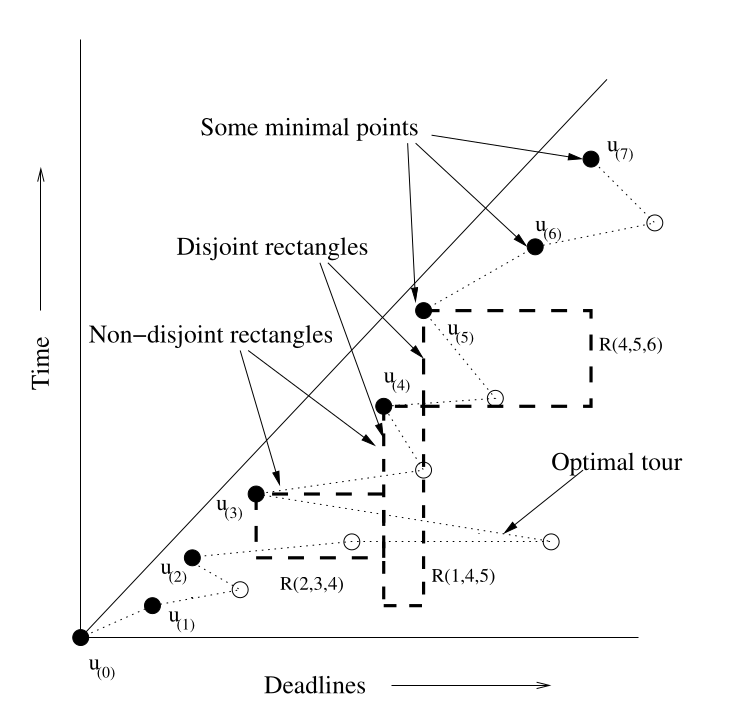
\includegraphics[scale=0.4]{images/TWTSP_rectangles.png}
	\caption{Γραφική αναπαράσταση minimal κόμβων σε σύστημα συντεταγμένων Deadline-Time \\ πηγή: Approximation Algorithms for Deadline-TSP and Vehicle Routing with Time-Windows \cite{12}}
\end{matlab}

\begin{matlab}
	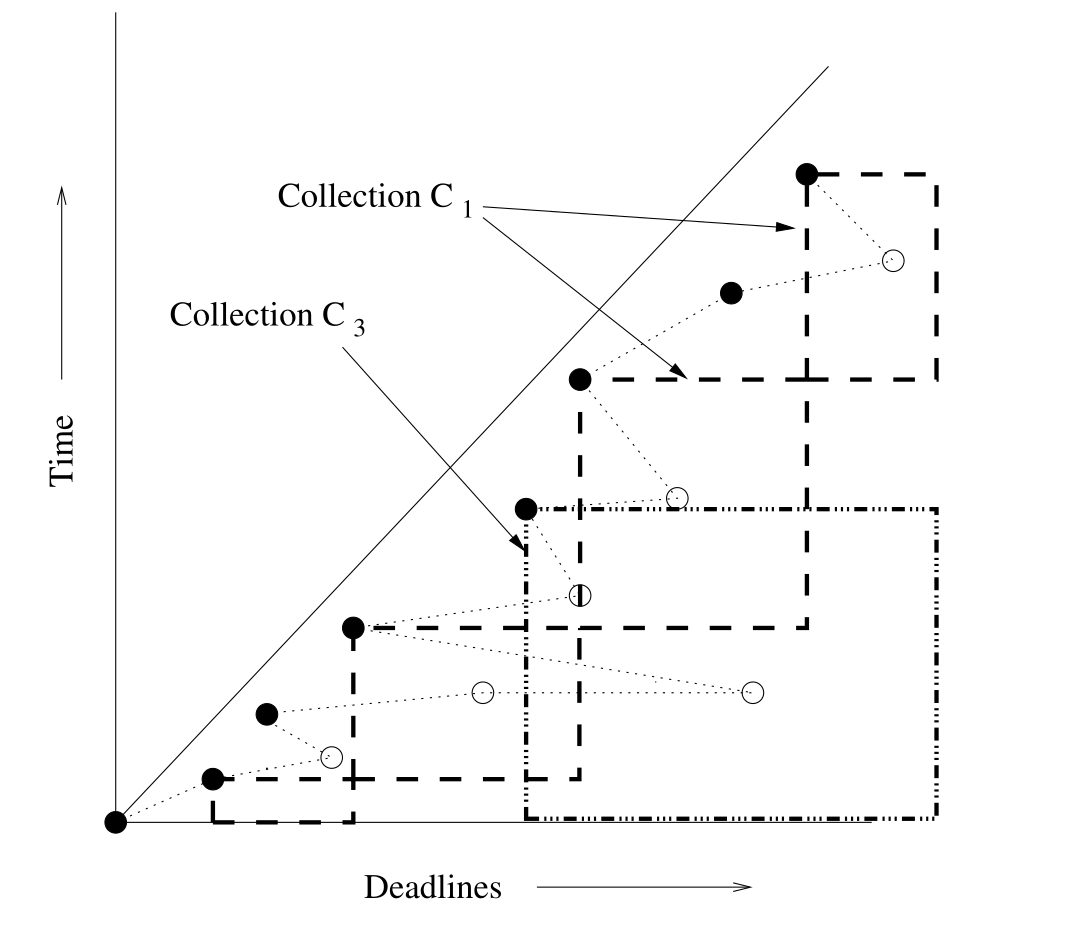
\includegraphics[scale=0.28]{images/TWTSP_disjoint.png}
	\caption{Γραφική αναπαράσταση minimal κόμβων σε σύστημα συντεταγμένων Deadline-Time και ξένα τετράγωνα\\ πηγή: Approximation Algorithms for Deadline-TSP and Vehicle Routing with Time-Windows \cite{12}}
\end{matlab}


Το ερώτημα τώρα είναι πόσο μεγάλο μπορεί να γίνει το \(i\). Για να βρόυμε το επιτρεπτό εύρος τιμών για το \(i\) πρέπει να ανατρέξουμε στο επιτρεπτό εύρος τιμών για το \(j\). όπως υποδεικνύει η σχέση (7.1) 

\begin{align*}
	-1 \leq j \leq 2^{\log m - i}
\end{align*}

Κοιτάζουμε το άνω φράγμα για το \(j\)

\begin{align*}
	2^{\log m - i} = 2^{\log m} \cdot 2^{-i} = \frac{m}{2^i}
\end{align*}

αν υποθέσουμε ότι το log έχει βάση το 2. Για προφανείς λόγους το άνω φράγμα του \(j\) πρέπει να είναι μεγαλύτερο της μονάδας, οποτε

\begin{align*}
	\frac{m}{2^i} & \geq 1 \Leftrightarrow \\
	m & \geq 2^i \Leftrightarrow \\
	i & \leq \log m
\end{align*}

Υποθέτουμε, λοιπόν, ότι έχουμε μια οικογένεια συλλογών από ξένα τετράγωνα \(F = {C_1,...,C_{\log m}}\).

\chapter{Results}

\chapter{Discussion and Future work}

\chapter{Acknowledgement}

\chapter{References}
\begin{thebibliography}{depth}
	\bibitem[1]{1}
	Exact and Approximation Algorithms for Time-Window TSP, 
	Jie Gao, Su Jia, Joseph S. B. Mitchell,
	CG:YRF, Boston, MA, USA, June 14-18, 2016
	
	\bibitem[2]{2}
	An Optimal Lower Bound for the Hilbert-type, Planar Universal Traveling Salesman Problem, 
	Patrick Eades, Julián Mestre,
	CG:YRF, Brisbane, Australia, July 4-7, 2017
	
	\bibitem[3]{3}
	The Geometric Maximum Traveling Salesman Problem, 
	David S. Johnson, Arie Tamir,
	Article in Journal of the ACM · May 2002
	
	\bibitem[4]{4}
	Εισαγωγή στους αλγορίθμους, Δεύτερη έκδοση, 
	Thomas H. Cormen, Charles E. Leiserson, Ronald L. Rivest, Clifford Stein,
	Πανεπιστημιακές εκδόσεις Κρήτης, 2011,
	ISBN: 978-960-524-473-6
	
	\bibitem[5]{5}
	Τεχνητή Νοημοσύνη, Μία σύγχρονη προσέγγιση, Δεύτερη Αμερικανική έκδοση, 
	Stuart Russel, Peter Norvig,
	σελ.: 101,
	Κλειδάριθμος 2005,
	ISBN: 960-209-873-2
	
	\bibitem[6]{6}
	Στοιχεία διακριτών μαθηματικών, 
	C. L. Liu,
	σελ.: 171-172, 178-179, 190-201,
	Πανεπιστημιακές εκδόσεις Κρήτης 2014, 
	ISBN: 978-960-524-072-1	
	
	\bibitem[7]{7}
	Discrete and Computational Geometry, 
	Satyan L. Devadoss, Joseph O'Rourke,
	σελ.: 81-86,
	Princeton University Press, 2011, 
	ISBN: 978-0-691-14553-2
	
	\bibitem[8]{8}
	Computational Geometry,	Algorithms and Applications, Third Edition, 
	Mark de Berg, Otfried Cheong, Marc van Kreveld, Mark Overmars,
	σελ.: 193-204,
	Springer, 2008, 
	ISBN: 978-3-540-77973-5
	
	\bibitem[9]{9}
	Υπολογιστική Γεωμετρία: Μια σύγχρονη αλγοριθμική προσέγγιση, 
	Γιάννης Ζ. Εμίρης,
	σελ.: 199-208,
	Κλειδάριθμος, 2008, 
	ISBN: 978-960-461-141-6 
	
	\bibitem[10]{10}
	An O ( n log n ) Heuristic for the Euclidean Traveling Salesman Problem, 
	Evgeny Yanenko, Eckart
	Schuhmacher, Ulrich Spörlein, Kurt Tutschku,
	April 25, 2005
	
	\bibitem[11]{11}
	Applications of the TSP,
	http://www.math.uwaterloo.ca/tsp/apps/index.html
	
	\bibitem[12]{12}
	Approximation Algorithms for Deadline-TSP and Vehicle Routing with Time-Windows,
	N. Bansal, A. Blum, S. Chawla, and A. Meyerson,
	In Proceedings of the Thirty-sixth Annual ACM Symposium on Theory of Computing,
	STOC ’04, pages 166–174, 2004
	
	\bibitem[13]{13}
	Good triangulations yield good tours,
	Adam N. Letchford, Nicholas A. Pearson,
	Department of Management Science, Lancaster University, Lancaster LA1 4YW, UK, 
	4 May 2006

	\bibitem[14]{14}
	Σχεδίαση και Ανάλυση Αλγορίθμων,
	Κωνσταντίνος Τσίχλας, Ιωάννης Μανωλόπουλος, Αναστάσιος Γούναρης,
	σελ.: 317-320,
	http://repfiles.kallipos.gr/html\_books/4410/contents.html ,2015
	ISBN: 978-960-603-465-7
	
	
\end{thebibliography}
\end{document}